% appendix.tex
% Supplementary material: empirical validations of assumptions used in
% the main-text derivations, plus material that is too dense for the
% main body but useful for replication.
%
% Language-audit pass, 2026-07-14 (see project_language_audit_2026-07-14
% memory; final section of the pass). Kept every algebra step (no
% collapsed align blocks) but cut narrating prose around them ("we
% expand this in two stages", "distributing", "pulling outside the
% sums"). Killed generic terminology: "artifact" -> "bias" (matches
% discussion.tex's "diversification-return bias"; the one surviving
% "sample-size artifact" is a standard statistical idiom, kept
% consistent with results.tex), "anchor"/"anchoring" -> literal
% ("set from", "matching"), "engine"/"engine-raw" -> "raw" (was
% implementation jargon for the uncorrected ensemble; also renamed the
% $W_{\mathrm{engine}}$ subscript to $W_{\mathrm{raw}}$), "operating
% point" -> "parameter values"/"fitted", "pipeline"/"framework" ->
% "construction"/"procedure", generic "mechanism" -> literal (e.g. "the
% persistence mechanism" -> "the duration model"), "downstream" cut,
% "smoke test" cut (software-testing jargon), "composer" -> "composition
% method" (last file needing this swap; done everywhere now), "sat/sits"
% -> "clustered"/"remained near"/"falls". Table 3 caption's "Clipping is
% a stability mechanism" rewritten to state the observed result
% directly, per the audit's own suggested rewrite.

\section{Empirical cross-term diagnostic}
\label{sec:supp-cov}

The variance correction of Eq.~\eqref{eq:scale} assumes
$\Cov(\tg_i^{\mathrm c},g_m)\approx0$, allowing the variance derivation to omit
the cross-term. This assumption does not follow automatically from
the fitting procedure because each JumpHMM uses the asset's full
growth-rate history, including its market-correlated component. A
remaining market loading in the generator draw would invalidate the
closed-form scale. We tested the assumption by sampling $R = 100$
generator growth-rate paths $\tg_i^{(r)}$ per ticker from each
generator and computing the normalized cross-covariance against the real
return path for a broad-market exchange-traded fund (ticker SPY):
\begin{equation}
  \mathrm{cov}^{\mathrm{norm}}_i
  = \frac{1}{R} \sum_{r=1}^{R}
    \frac{\Cov((\tg_i^{(r)})^{\mathrm c},\, g_m)}{\sigma_{\gen,i}\, \sigma_m}.
\end{equation}
Centering does not change covariance, so these values are numerically
identical to those obtained from the raw draws.
We plotted the per-ticker values as histograms
(Fig.~\ref{fig:cov_diag}). Across the $423$ tickers, the full-return
JumpHMM generator (used by the hybrid and naive composition
methods), the residual-fit JumpHMM generator (used by the
JumpHMM-on-residuals composition method), and the Gaussian baseline
had universe-mean normalized cross-covariances of $1.53\times10^{-4}$,
$6.58\times10^{-5}$, and $2.26\times10^{-4}$, respectively. Their
per-ticker values ranged from $-0.0061$ to $0.0061$. These values
quantify the cross-term omitted in Eq.~\eqref{eq:scale}.

\begin{figure}[H]
  \centering
  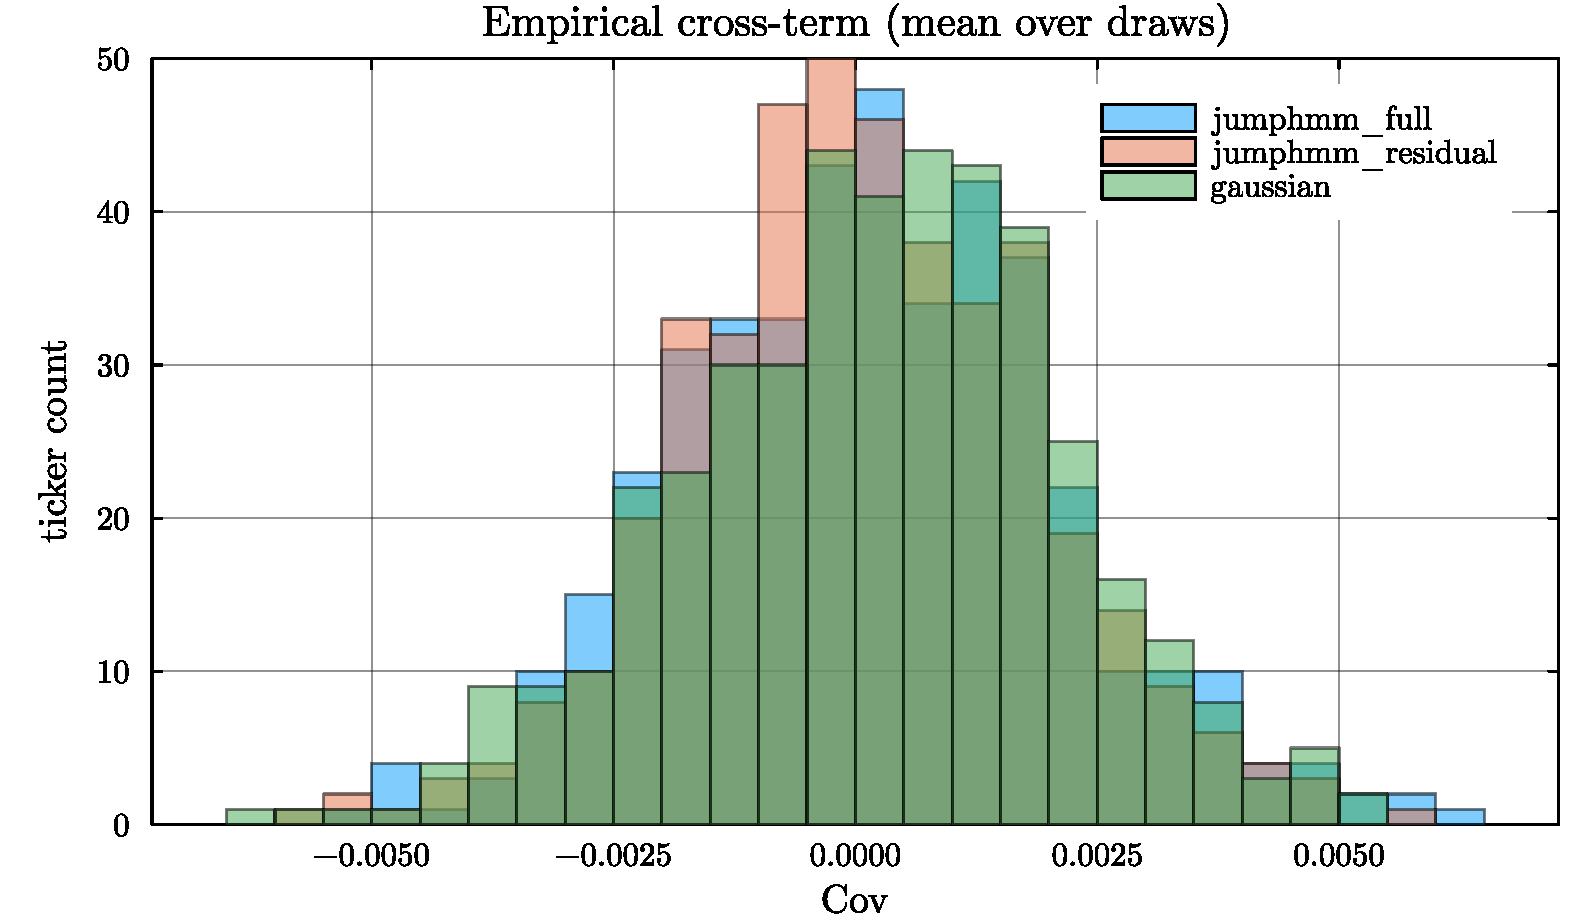
\includegraphics[width=0.85\textwidth]{figs/supplement/FigS01-Cross-Covariance.pdf}
  \caption{\textbf{Empirical normalized cross-covariance
    $\Cov(\tg_i^{\mathrm c}, g_m) / (\sigma_{\gen,i}\, \sigma_m)$ across
    the $423$-ticker universe.} Histograms were stacked per generator,
    with each per-ticker value averaged over $R = 100$ generator
    growth-rate paths. Universe means were $1.53\times10^{-4}$,
    $6.58\times10^{-5}$, and $2.26\times10^{-4}$ for the full-return
    JumpHMM, residual-fit JumpHMM, and Gaussian generators.}
  \label{fig:cov_diag}
\end{figure}

% =============================================================================
% S2  Bias correction for daily-rebalanced backtests
% Four flat paragraphs:
%   (1) origin of the bias (Booth-Fama identity + iid residuals)
%   (2) empirical demonstration on a 20-asset allocator
%   (3) the location-shift correction (formula, prior, validation check)
%   (4) rejected alternatives
% =============================================================================

\section{Rebalancing under independent residuals}
\label{sec:supp-bias}

To determine what a portfolio-level use of these paths inherits from
the independent-residual construction, this appendix derives the
diversification return of a rebalanced portfolio under
Eq.~\eqref{eq:sim-composition}. The variance correction in
Eq.~\eqref{eq:scale} sets each synthetic asset's second moment to its
generator target. When that target matches the empirical second
moment, the second-order formula for the diversification return is
matched at the asset level as well. What the construction does not
match is the cross-asset residual covariance, and the derivation below
isolates where that omission enters.

The synthetic paths reproduce per-asset marginals and single-factor
cross-sectional dependence. Each residual generator retains its own
temporal structure, but the residual paths are generated independently
across assets at each date. The construction therefore omits
cross-asset residual covariance. Consider a
daily-rebalanced portfolio of $N$
assets with constant target weights $w_i \ge 0$, $\sum_i w_i = 1$,
reset to those weights at the start of each trading day. Throughout
this derivation $g_i(t)$ is the annualized log-growth rate of
Eq.~\eqref{eq:growth_rate}, so the per-period log return on asset
$i$ is $g_i(t)\,\Delta t$ with $\Delta t = 1/252$~yr. The wealth
process is:
\begin{equation}
  W_t \;=\; W_{t-1} \sum_{i} w_i \exp\!\big(g_i(t)\,\Delta t\big),
  \label{eq:wealth-recursion}
\end{equation}
so the per-step log return on the portfolio is
$\log(W_t/W_{t-1}) = \log\!\sum_i w_i \exp(g_i(t)\,\Delta t)$. We
suppress the time argument, writing $g_i$ for $g_i(t)$. A
second-order Taylor expansion of the exponential about zero is
$\exp(g_i\,\Delta t) = 1 + g_i\,\Delta t + \tfrac{1}{2}(g_i\,\Delta t)^2
+ O((g\,\Delta t)^3)$. Substituting it into each summand of
$\sum_i w_i \exp(g_i\,\Delta t)$ gives:
\begin{align}
  \sum_{i} w_i \exp\!\big(g_i\,\Delta t\big)
   &= \sum_{i} w_i \!\left[\,1 + g_i\,\Delta t
        + \tfrac{1}{2}(g_i\,\Delta t)^2
        + O\!\big((g\,\Delta t)^3\big)\right]
       && \text{(Taylor)} \notag \\
   &= \sum_{i} w_i
        + \Delta t \sum_{i} w_i\, g_i
        + \tfrac{1}{2}(\Delta t)^2 \sum_{i} w_i\, g_i^2
        + O\!\big((g\,\Delta t)^3\big)
       && \text{(distribute)} \notag \\
   &= 1 + \Delta t \sum_{i} w_i\, g_i
        + \tfrac{1}{2}(\Delta t)^2 \sum_{i} w_i\, g_i^2
        + O\!\big((g\,\Delta t)^3\big).
       && \text{(}\textstyle\sum_i w_i = 1\text{)}
  \label{eq:exp-expand}
\end{align}
A second-order Taylor expansion of $\log(1+x)$ about $x=0$ gives
$\log(1+x) = x - \tfrac{1}{2}x^2 + O(x^3)$. Identifying $1 + x$ with
the right-hand side of Eq.~\eqref{eq:exp-expand}, the order-$\Delta t$
correction is
$x := \Delta t \sum_i w_i\, g_i + \tfrac{1}{2}(\Delta t)^2 \sum_i w_i\, g_i^2$,
and squaring keeps only the leading $(\Delta t)^2$ term:
$x^2 = (\Delta t)^2 (\sum_i w_i\, g_i)^2 + O((\Delta t)^3)$ because
the cross term has an extra $\Delta t$ factor. Substitution gives:
\begin{align}
  \log\!\frac{W_t}{W_{t-1}}
   &= \log\!\Big(1 + x + O\!\big((g\,\Delta t)^3\big)\Big) \notag \\
   &= x - \tfrac{1}{2}\, x^2 + O\!\big(x^3\big) \notag \\
   &= \Delta t \sum_{i} w_i\, g_i
        + \tfrac{1}{2}(\Delta t)^2 \sum_{i} w_i\, g_i^2
        \notag \\
   &\quad - \tfrac{1}{2}(\Delta t)^2
        \!\Big(\sum_{i} w_i\, g_i\Big)^{\!2}
        + O\!\big((g\,\Delta t)^3\big) \notag \\
   &= \Delta t \sum_{i} w_i\, g_i
        + \tfrac{1}{2}(\Delta t)^2 \!\left[\sum_{i} w_i\, g_i^2
        \right. \notag \\
   &\hspace{8em}\left.{}- \Big(\sum_{i} w_i\, g_i\Big)^{\!2}\right]
        + O\!\big((g\,\Delta t)^3\big).
  \label{eq:rp-taylor}
\end{align}
Dividing through by $\Delta t$ extracts the portfolio's annualized
one-step log-growth rate $g_p(t) := \Delta t^{-1}\log(W_t/W_{t-1})$,
the portfolio counterpart of the per-asset $g_i(t)$ (still
suppressing the time argument):
\begin{equation}
  g_p \;=\; \sum_{i} w_i\, g_i
   \;+\; \tfrac{1}{2}\,\Delta t \!\left(\sum_{i} w_i\, g_i^2
        \;-\; \Big(\sum_{i} w_i\, g_i\Big)^{\!2}\right)
   \;+\; O\!\big((\Delta t)^2\big).
  \label{eq:gp-onestep}
\end{equation}

To obtain expected annualized portfolio growth, we restored the time
argument and took unconditional expectations of
Eq.~\eqref{eq:gp-onestep} under stationarity. Define the
per-asset annualized mean and variance:
\begin{equation}
  \mu_i \;:=\; \E\!\big(g_i(t)\big), \qquad
  \sigma_i^2 \;:=\; \Var\!\big(g_i(t)\big),
\end{equation}
the per-rate covariance
$\Sigma_{ij} := \Cov\!\big(g_i(t), g_j(t)\big)$, and the per-rate
portfolio variance
$\sigma_p^2 := \Var\!\big(\textstyle\sum_i w_i g_i(t)\big) =
w^\top \Sigma w$. The $O(\Delta t)$ correction in
Eq.~\eqref{eq:gp-onestep} contains two squared quantities,
$\sum_i w_i\, g_i(t)^2$ and $(\sum_i w_i\, g_i(t))^2$. Both expand
by the second-moment identity, which holds for any random variable
$X$ with finite second moment:
\begin{equation}
  \E\!\big(X^2\big) \;=\; \E\!\big(X\big)^2 \;+\; \Var(X).
  \label{eq:second-moment}
\end{equation}
Applying this identity to $X = g_i(t)$ and summing against $w_i$ gives:
\begin{align}
  \E\!\Big(\sum_{i} w_i\, g_i(t)^2\Big)
   &\;=\; \sum_{i} w_i\, \E\!\big(g_i(t)^2\big)
       && \text{(linearity)} \notag \\
   &\;=\; \sum_{i} w_i\!\left[\,\mu_i^2 + \sigma_i^2\,\right]
       && \text{(by Eq.~\eqref{eq:second-moment})} \notag \\
   &\;=\; \sum_{i} w_i\, \mu_i^2 \;+\; \sum_{i} w_i\, \sigma_i^2.
   \label{eq:exp-gi2}
\end{align}
Applying the identity to $X = \sum_i w_i g_i(t)$, whose mean is
$\sum_i w_i\mu_i$ and whose variance is $\sigma_p^2$, gives:
\begin{align}
  \E\!\Big(\Big(\textstyle\sum_{i} w_i g_i(t)\Big)^{\!2}\Big)
   &\;=\; \E\!\Big(\textstyle\sum_{i} w_i g_i(t)\Big)^{\!2}
       \;+\; \Var\!\Big(\textstyle\sum_{i} w_i g_i(t)\Big)
       && \text{(by Eq.~\eqref{eq:second-moment})} \notag \\
   &\;=\; \Big(\textstyle\sum_{i} w_i\, \mu_i\Big)^{\!2}
       \;+\; \sigma_p^2.
   \label{eq:exp-sum2}
\end{align}
We substituted Eqs.~\eqref{eq:exp-gi2}--\eqref{eq:exp-sum2} into the
expectation of Eq.~\eqref{eq:gp-onestep} and grouped the variance and
mean contributions as follows:
\begin{equation}
\begin{aligned}
  \E(g_p) \;={}& \sum_{i} w_i\, \mu_i
  + \underbrace{\tfrac{1}{2}\,\Delta t\!\left(\sum_{i} w_i\, \sigma_i^2
       - \sigma_p^2\right)}_{\displaystyle D} \\
  &+ \tfrac{1}{2}\,\Delta t\!\left[\sum_{i} w_i\, \mu_i^2
       - \Big(\sum_{i} w_i\, \mu_i\Big)^{\!2}\right]
  + O\!\big((\Delta t)^2\big),
\end{aligned}
  \label{eq:booth-fama}
\end{equation}
the Booth-Fama identity for the daily-rebalanced portfolio in
annualized growth-rate units \cite{boothFama1992,
markowitz1976longRun}. The middle term, $D$, is the diversification
return: the $O(\Delta t)$ correction equal to half the difference
between the weighted-average per-asset variance $\sum_i w_i \sigma_i^2$
and the portfolio variance $\sigma_p^2$. The per-rate
moments $\mu_i$ and $\sigma_i^2$
have units $\mathrm{yr}^{-1}$ and $\mathrm{yr}^{-2}$ respectively;
the products $\Delta t\,\sigma_i^2$ and $\Delta t\,\sigma_p^2$ in
Eq.~\eqref{eq:booth-fama} are the annualized variances
($\mathrm{yr}^{-1}$). The
third term in Eq.~\eqref{eq:booth-fama} is the cross-sectional
dispersion of the per-asset annualized means, of order
$\Delta t\,\mu^2 \sim 3\!\times\!10^{-5}~\mathrm{yr}^{-1}$ at
$\mu \sim 0.08~\mathrm{yr}^{-1}$ and negligible against the
variance term $D \sim \Delta t\,\sigma^2 \sim 4\!\times\!10^{-2}~
\mathrm{yr}^{-1}$; we drop it. The realized annualized compound
growth rate $\bar g_p = (T\,\Delta t)^{-1}\log(W_T/W_0) =
T^{-1}\sum_{t} g_p(t)$ converges to $\E(g_p)$ by the ergodic
theorem under any stationary residual process, so the long-run
limit is fixed by the one-time-slice unconditional joint
distribution of $(g_i(t))_i$ and does not, in itself, depend on
the serial structure of the residual draw.

To rewrite $D$ in a form that makes its non-negativity manifest,
expand $\sigma_p^2 = \sum_i w_i^2 \sigma_i^2 + 2 \sum_{i<j} w_i w_j
\Sigma_{ij}$ and use the identity $\sum_i w_i (1 - w_i) \sigma_i^2 =
\sum_{i<j} w_i w_j (\sigma_i^2 + \sigma_j^2)$ that holds for any
weights summing to one:
\begin{equation}
  D \;=\; \tfrac{1}{2}\,\Delta t\!\left(\sum_i w_i \sigma_i^2 - \sigma_p^2\right)
  \;=\; \tfrac{1}{2}\,\Delta t \sum_{i<j} w_i w_j \,\Var(g_i - g_j) \;\ge\; 0,
  \label{eq:dr-pairwise}
\end{equation}
so $D$ equals one-half the annualized weighted-average pairwise
growth-rate-difference variance and is therefore non-negative, with equality only when every
pair $(i,j)$ comoves perfectly ($\Var(g_i - g_j) = 0$) or all weight
concentrates on a single asset. The rebalancing rule itself produces
this effect: weights drift between rebalances, the rebalancer sells
whatever has outperformed (its weight rose above target) and buys
whatever has underperformed (its weight fell below target), and the
trade systematically converts period-by-period cross-sectional
dispersion into compounded growth. Markowitz
\cite{markowitz1976longRun} described this as the variance bonus of
the long-run mean-variance allocation; Booth and Fama
\cite{boothFama1992} called it the diversification return.

To separate market and residual contributions to the diversification
return, we substituted the single-index decomposition
$g_i(t) = \alpha_i + \beta_i\, g_m(t) + \eps_i(t)$, with market
variance $\sigma_m^2 := \Var(g_m(t))$, per-asset residual variance
$\sigma_{\eps,i}^2 := \Var(\eps_i(t))$, and
$\Cov(g_m, \eps_i) = 0$ (verified in
Sec.~\ref{sec:supp-cov}), into Eq.~\eqref{eq:dr-pairwise} gives:
\begin{equation}
  \Var(g_i - g_j) \;=\; (\beta_i - \beta_j)^2 \sigma_m^2
  \;+\; \Var(\eps_i - \eps_j),
\end{equation}
Because $g_m$ and the residuals are uncorrelated, this relation splits
the diversification return into market-beta-dispersion and
idiosyncratic components:
\begin{equation}
  D \;=\;
  \underbrace{\tfrac{1}{2}\,\Delta t\,\sigma_m^2 \sum_{i<j} w_i w_j (\beta_i - \beta_j)^2}_{D_{\mathrm{mkt}}}
  \;+\;
  \underbrace{\tfrac{1}{2}\,\Delta t \sum_{i<j} w_i w_j \,\Var(\eps_i - \eps_j)}_{D_\eps},
  \label{eq:dr-sim}
\end{equation}
where the market-beta-dispersion component $D_\mathrm{mkt}$ equals
$\tfrac{1}{2}\,\Delta t\,\sigma_m^2 [\sum_i w_i \beta_i^2 -
(\sum_i w_i \beta_i)^2]$, the weighted cross-sectional $\beta$
dispersion scaled by the annualized market variance
$\Delta t\,\sigma_m^2$. Across the $423$-ticker universe the empirical
$\beta$ distribution spans $[0.03, 1.79]$ with interquartile range
$[0.81, 1.18]$ and the SPY annualized variance
$\Delta t\,\sigma_m^2 \approx 0.04~\mathrm{yr}^{-1}$. The weighted
variance of $\beta$ is bounded by one quarter of its squared range,
so $D_{\mathrm{mkt}}$ is at most $0.016~\mathrm{yr}^{-1}$, or $1.6$
percentage points per year over this universe. For the idiosyncratic
component $D_\eps$, residuals were approximately orthogonal across
assets at the same time slice. Therefore,
$\Var(\eps_i - \eps_j) \approx \sigma_{\eps,i}^2 + \sigma_{\eps,j}^2$,
and $D_\eps$ scales with the weighted-average annualized idiosyncratic
variance $\Delta t\,\sigma_{\eps,i}^2$ per name.

The second-order value of $D$ depends on same-time unconditional
moments, not on serial dependence. Equation~\eqref{eq:scale} sets
$\sigma_{\gen,i}^2=\beta_i^2\sigma_m^2+\sigma_{\eps,i}^2$ to its
empirical target. Any residual generator with the same unconditional
second moments therefore gives the same $D$. This includes a stationary
first-order autoregressive [AR(1)] residual generator
$\eps_i(t) = \phi\, \eps_i(t-1) + \eta_i(t)$ with independent and
identically distributed innovations $\eta_i$ tuned so that
$\Var(\eps_i) = \sigma_{\eta,i}^2 / (1 - \phi^2) = \sigma_{\eps,i}^2$.
The parameter $\phi$ leaves the marginal distribution at a single
time slice unchanged. It therefore does not change $\E(g_p)$ in
Eqs.~\eqref{eq:booth-fama} and~\eqref{eq:dr-sim}, but it changes
sampling variance. For a stationary AR(1) residual with variance
$\sigma_\eps^2$, the variance of its sample mean is approximately
$T^{-1}\sigma_\eps^2(1+\phi)/(1-\phi)$. Under ergodicity, serial
dependence changes per-path sampling noise, not the stationary mean.
Serial dependence in the residual draw is therefore not a lever on the
diversification return at the level of the second-order formula.

The direct structural difference is contemporaneous. The derivation
assumes residuals are orthogonal across assets at each time slice, as
they are in the independent per-asset generator. Real residuals share
sector and style factors, which reduce $\Var(\eps_i-\eps_j)$ below the
independent-generator value
$\sigma_{\eps,i}^2+\sigma_{\eps,j}^2$. Matching each marginal variance
does not restore this covariance. The synthetic $D_\eps$ will therefore
exceed its real-market counterpart when the omitted covariance is
positive. Quantifying that contribution requires a joint-residual
experiment with the marginals and the allocation rule held fixed,
which we did not run. Realized diversification returns on real equity
portfolios are also attenuated relative to the second-order formula at
all rebalancing horizons~\cite{boucheyNemtchinovWong2015}, so the
synthetic excess is an upper bound on what an independent-residual
generator would contribute in a live comparison.


% =============================================================================
% S3 Validation metric definitions (KS, AD, W1, Hellinger)
% =============================================================================

\section{Validation metric definitions}
\label{sec:supp-validation}

To make the validation criteria reproducible, we defined the
distributional and tail metrics reported in the main results. The
two-sample Kolmogorov--Smirnov (KS) statistic
between the empirical cumulative distribution functions (CDFs) of
the observed and simulated growth-rate samples ($G_{\rm obs}$ of length $n$ and $G_{\rm sim}$ of length $m$)
is $D = \sup_x |F_n(x) - F_m(x)|$ \cite{kolmogorov1933, smirnov1948};
the test rejects when $D$ exceeds the critical value at level
$\alpha = 0.05$. The Anderson--Darling (AD) statistic places greater weight
on the tails via the integral
$A^2 = nm/(n+m) \int [F_n(x) - F_m(x)]^2 / [F(x)(1-F(x))] \, dF(x)$,
where $F$ is the pooled empirical CDF \cite{andersonDarling1952}. The
Wasserstein-$1$ distance between two empirical distributions of equal
length is the average of sorted-quantile differences:
\begin{equation}
W_1 = \frac{1}{n} \sum_{i=1}^{n} \big| G_{\rm obs}^{(i)} - G_{\rm sim}^{(i)} \big|,
\label{eq:wasserstein}
\end{equation}
with $G^{(i)}$ the $i$th order statistic. The Hill upper-tail index is the classical
order-statistic estimator:
\begin{equation}
\hat\xi = \frac{1}{k-1} \sum_{i=1}^{k-1}
  \log\!\left( \frac{X_{(i)}}{X_{(k)}} \right),
\label{eq:hill}
\end{equation}
with $X_{(1)} \ge X_{(2)} \ge \dots$ the ordered upper-tail
absolute returns; $k$ is set to the upper $5\%$ of the
sample. For a Pareto-tailed distribution with shape $\alpha$,
$\hat\xi \approx 1/\alpha$. For the Hellinger calculation, we binned
both samples on a common grid and normalized the bin counts to
probability masses $p$ and $q$. Their distance is:
\begin{equation}
H(p, q) = \frac{1}{\sqrt{2}} \, \Big\| \sqrt{p} - \sqrt{q} \Big\|_2
\;\in\; [0, 1],
\label{eq:hellinger}
\end{equation}
with $H = 0$ for identical probability masses and $H = 1$ for
disjoint supports.

We abbreviate mean absolute error in the autocorrelation function as ACF-MAE.

% --- Figure: Statistical validation of HMM-WJ ---
\begin{figure}[H]
  \centering
  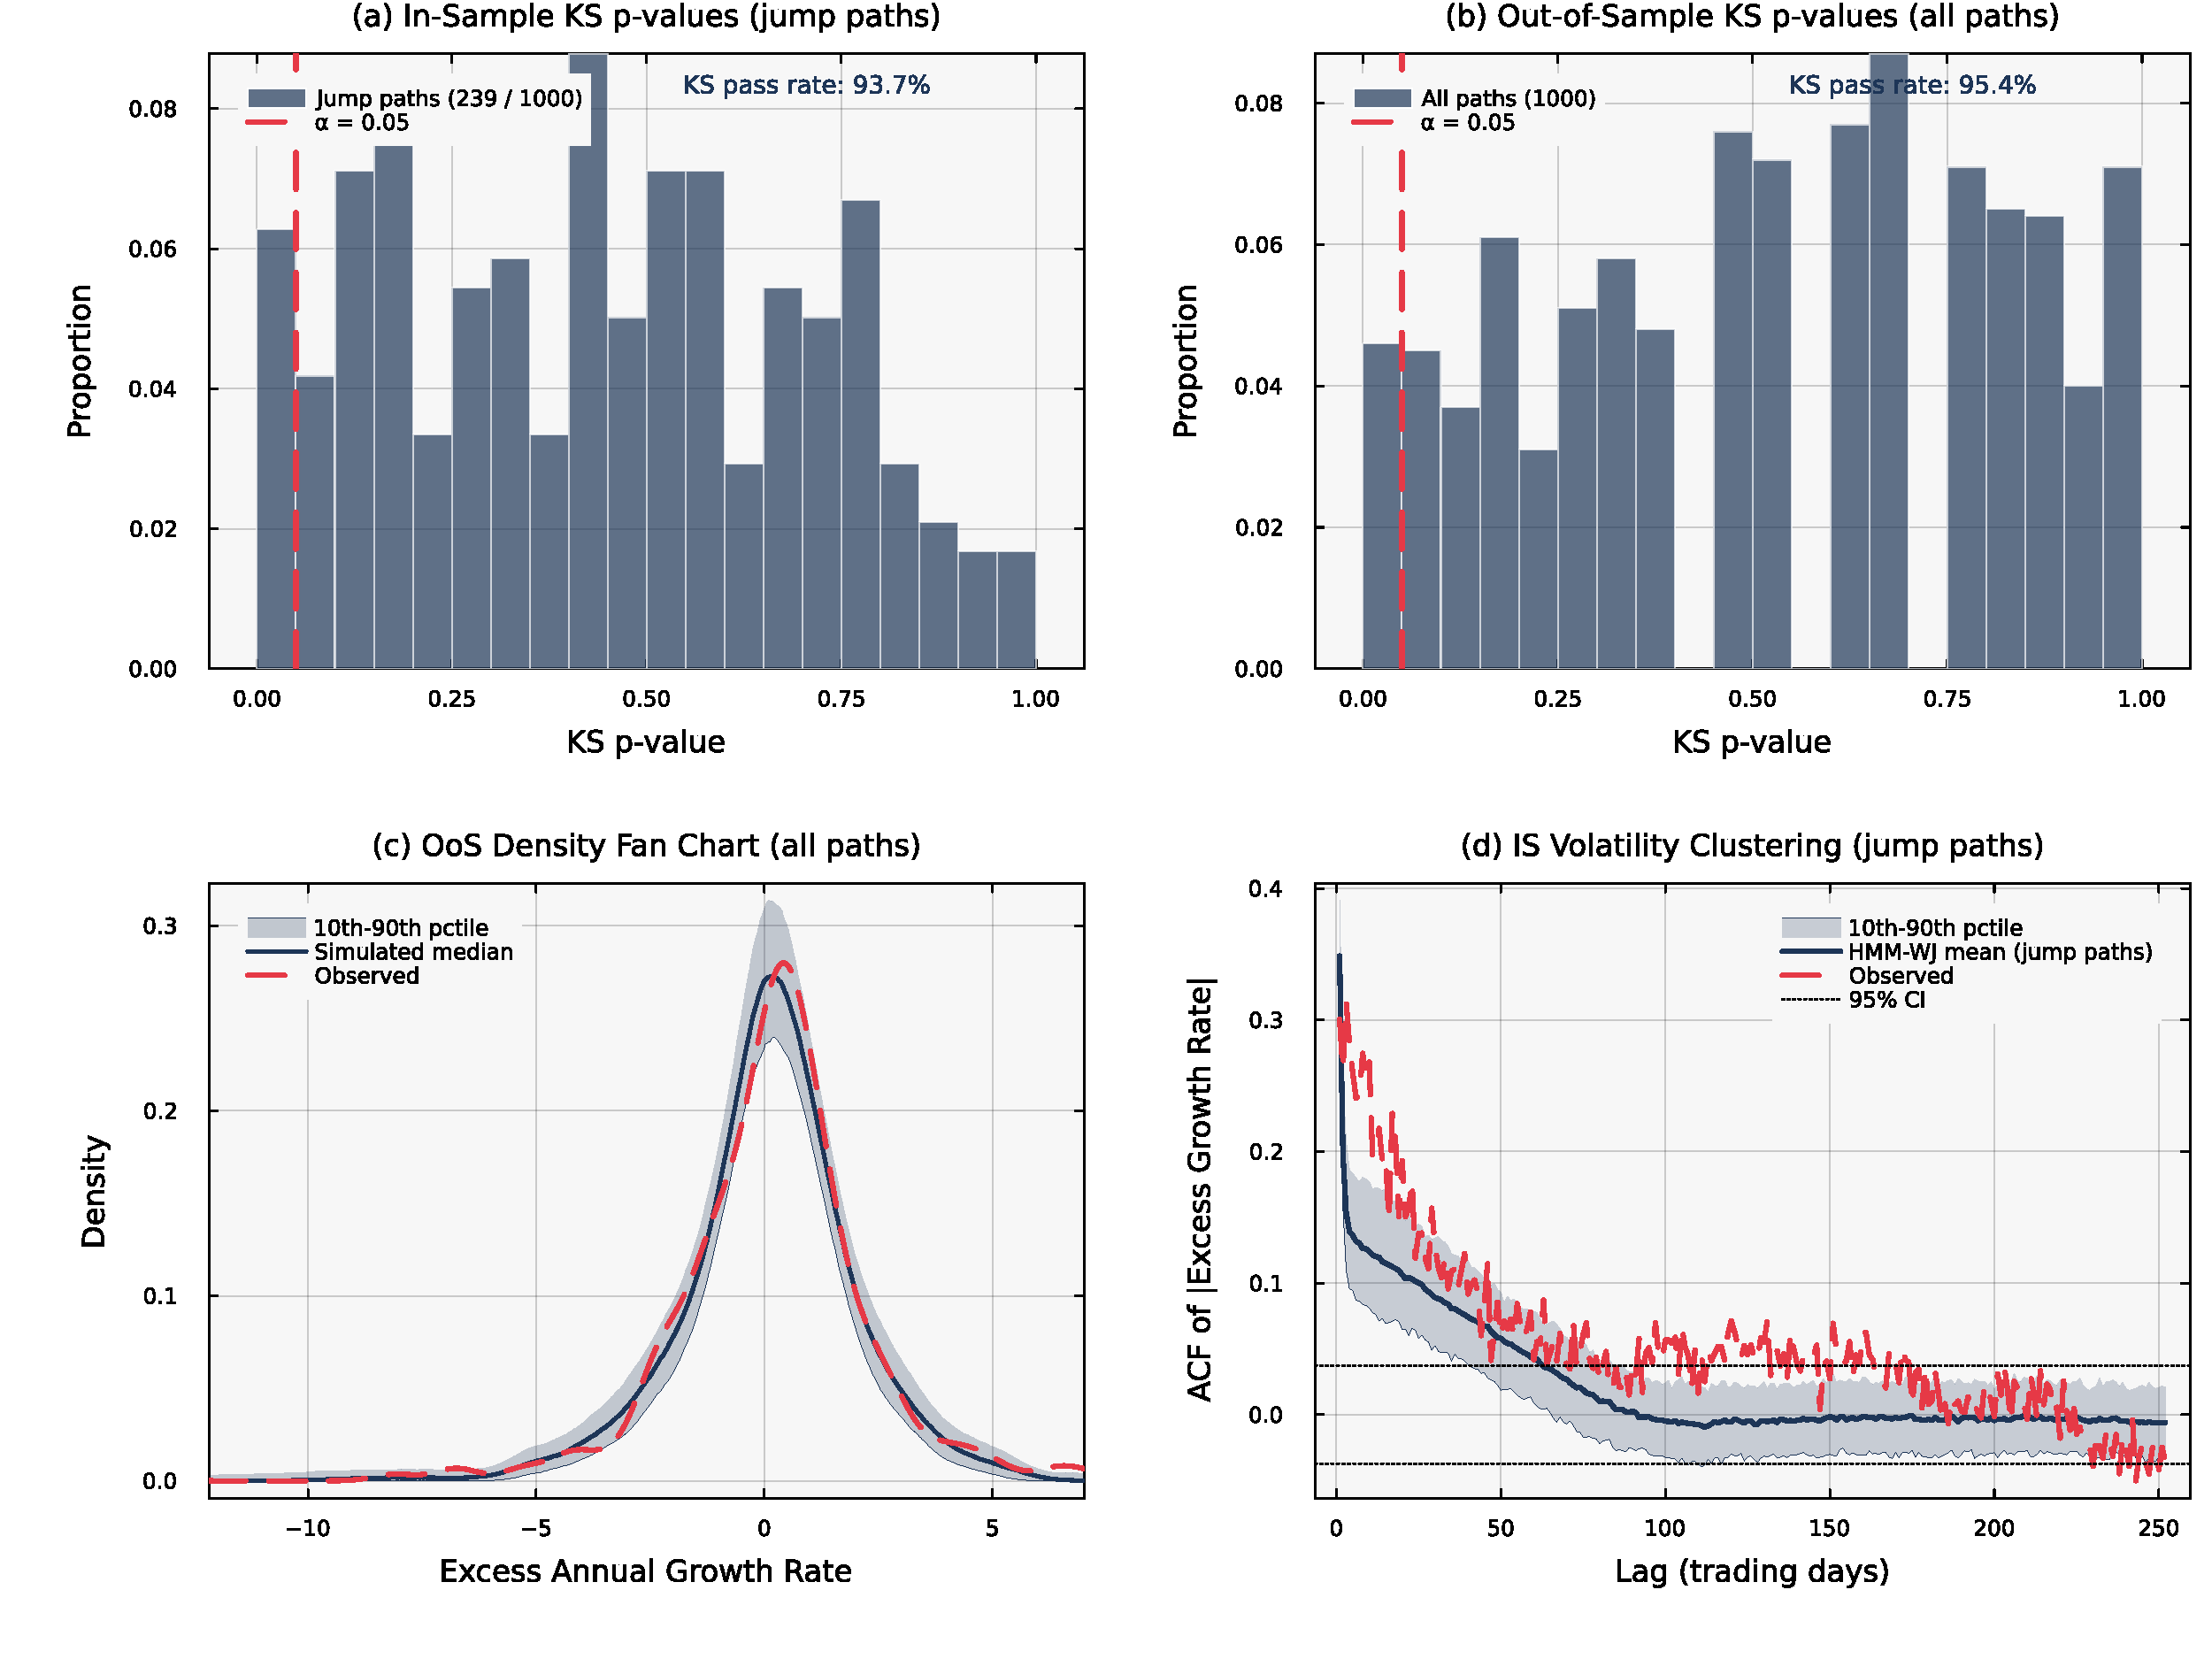
\includegraphics[width=\textwidth]{figs/supplement/FigS04-Statistical-Validation.pdf}
  \caption{\textbf{Statistical validation of the hidden Markov model with
    jumps (HMM-WJ)} ($N = 100$,
    $\alpha = 0.05$). Panels (a) and (d) condition on the
    $\sim\!24\%$ of in-sample paths containing jump events. (a)~In-sample
    KS $p$-values for $239$ jump paths (pass rate $93.7\%$). (b)~Out-of-sample
    KS $p$-values for all $1{,}000$ paths (pass rate $95.4\%$). (c)~Out-of-sample
    density fan chart; the observed density falls within the simulation
    envelope. (d)~Observed and mean simulated in-sample autocorrelation
    function (ACF) of $|G_t|$
    for jump paths.}
  \label{fig:statistical_validation}
\end{figure}

% =============================================================================
% S4  Derivation of the single-asset generator
% Six subsections: generative law; estimators; stationary law and moments;
% dependence without jumps; jump-episode arithmetic; what (epsilon, lambda)
% control. Every numerical value evaluates the stated closed form at the
% fitted SPY model (generator script: code/spy-experiment/SI-Derivation-Checks.jl).
% =============================================================================

% --- Table: SPY descriptive statistics ---
\begin{table}[H]
\centering
\caption{\textbf{Descriptive statistics and stylized-facts tests for
    SPY daily excess growth rates.} In-sample (IS): $2014$--$2024$
    ($T = 2{,}766$); out-of-sample (OoS): $2025$ ($T = 249$).
    Gaussian and Laplace columns show maximum likelihood estimation
    (MLE) fits to the in-sample data. We used the Jarque--Bera (JB)
    normality test and the Ljung--Box (LB) autocorrelation test at lag
    $20$. $^{\ast}$ denotes rejection at
    $\alpha = 0.05$.}
\label{tab:descriptive_stats}
\small
\begin{tabular}{@{}lcccc@{}}
\toprule
\textbf{Statistic} & \textbf{IS Observed} & \textbf{OoS Observed} & \textbf{Gaussian} & \textbf{Laplace} \\ \midrule
Mean (annualized, \%)       & 6.31   & 11.60  & 6.31   & 14.19  \\
Standard deviation of $G_t$ (\% yr$^{-1}$) & 214.50 & 220.62 & 214.46 & 205.93 \\
Skewness                    & $-0.753$ & $-1.093$ & 0    & 0      \\
Excess Kurtosis             & 7.715  & 6.867  & 0      & 3      \\
JB normality test           & reject$^\ast$ ($p<0.001$) & reject$^\ast$ ($p<0.001$) & not used & not used \\
LB test on $G_t$ (lag 20)   & reject$^\ast$ ($p<0.001$) & reject$^\ast$ ($p=0.019$) & not used & not used \\
LB test on $|G_t|$ (lag 20) & reject$^\ast$ ($p<0.001$) & reject$^\ast$ ($p<0.001$) & not used & not used \\
\bottomrule
\end{tabular}
\end{table}

\section{Derivation of the single-asset generator}
\label{sec:supp-generator}

This appendix derives the probability law of the fitted single-asset
generator and connects each fitted component to the empirical feature
it controls. The hidden Markov model with jumps (HMM-WJ), its no-jump
restriction (HMM-NJ), and their symbols follow the main-text
definitions in Eq.~\eqref{eq:emission} and
Algorithm~\ref{alg:hmmwj}. Unless noted otherwise, numerical values
evaluate the closed-form expressions at the fitted SPY model of
Table~\ref{tab:hyperparams}: $N = 100$ states, Student-$t$ degrees of
freedom $\nu = 5$, jump probability $\epsilon = 10^{-4}$, mean episode
duration $\lambda = 90$ steps, tail-selection probability
$p_{\rm neg} = 0.52$, tail-set size $N_{\rm tail} = 5$, and the
in-sample series of $T = 2{,}766$ daily excess growth rates.

\subsection{Generative law}
\label{sec:supp-gen-law}

The no-jump model generates a hidden state path $S_0, \dots, S_T$ on
$\{1, \dots, N\}$ and observations $G_1, \dots, G_T$ with the joint
density:
\begin{equation}
  p(s_0, \dots, s_T,\, g_1, \dots, g_T)
  \;=\; \bar\pi_{s_0} \prod_{t=1}^{T}
  \mathbf{T}_{s_{t-1},\, s_t}\; f_{s_t}(g_t),
  \label{eq:supp-joint-law}
\end{equation}
where $\bar\pi_{s_0}$ is the initial probability of state $s_0$,
$\mathbf{T}_{s_{t-1}, s_t}$ is the probability of moving from state
$s_{t-1}$ to state $s_t$, and $f_k$ is the emission density of state
$k$. Under Eq.~\eqref{eq:emission}, $f_k$ is the location-scale
Student-$t$ density:
\begin{equation}
  f_k(g) \;=\; \frac{1}{\sigma_k}\,
  \psi_\nu\!\left(\frac{g - \mu_k}{\sigma_k}\right),
  \qquad
  \psi_\nu(x) \;=\;
  \frac{\Gamma\!\big(\tfrac{\nu+1}{2}\big)}
       {\sqrt{\nu \pi}\; \Gamma\!\big(\tfrac{\nu}{2}\big)}
  \left(1 + \frac{x^2}{\nu}\right)^{\!-\frac{\nu+1}{2}},
  \label{eq:supp-emission-density}
\end{equation}
where $\psi_\nu$ is the density of a standard Student-$t$ random
variable with $\nu$ degrees of freedom, $\Gamma$ is the gamma
function, and $(\mu_k, \sigma_k)$ are the location and scale of state
$k$. The factorization in Eq.~\eqref{eq:supp-joint-law} states the
structural property that drives everything that follows: given the
state path, the observations are independent. Every form of serial
dependence the generator can produce must therefore be carried by the
state path~\cite{rabinerJuang1986}.

The jump-augmented model enlarges the hidden state. Let
$J_t \in \{0, 1, 2, \dots\}$ count the forced steps remaining after
time $t$, and let $u$ be the forced-step state distribution, which
mixes uniform draws over the two tail sets:
\begin{equation}
  u_k \;=\;
  \begin{cases}
    p_{\rm neg}/N_{\rm tail} & k \in \mathcal{S}_{-},\\[2pt]
    (1 - p_{\rm neg})/N_{\rm tail} & k \in \mathcal{S}_{+},\\[2pt]
    0 & \text{otherwise}.
  \end{cases}
  \label{eq:supp-u}
\end{equation}
Writing $p_K(m) = e^{-\lambda} \lambda^m / m!$ for the Poisson
probability of episode length $m$ and $\mathbf{1}\{\cdot\}$ for the
indicator function, the pair $(S_t, J_t)$ evolves by the transition
kernel:
\begin{equation}
\begin{aligned}
  &\Pr\big(S_t = k,\, J_t = j \mid S_{t-1} = s,\, J_{t-1} = i\big) \\
  &\qquad=\;
  \begin{cases}
    u_k\, \mathbf{1}\{j = i - 1\} & i \ge 1,\\[6pt]
    \big(1 - \epsilon + \epsilon e^{-\lambda}\big)\,
      \mathbf{T}_{s, k}\, \mathbf{1}\{j = 0\}
      \;+\; \epsilon\, p_K(j + 1)\, u_k & i = 0,
  \end{cases}
\end{aligned}
  \label{eq:supp-kernel}
\end{equation}
and the emission draw depends only on the first coordinate,
$G_t \sim f_{S_t}$. The two cases read as follows. While an episode is
active ($i \ge 1$), the next state is an independent draw from $u$ and
the counter decrements; the tail set and the state within it are
re-drawn at every forced step. While no episode is active ($i = 0$),
the chain either takes an ordinary transition (no trigger, or a
trigger whose Poisson draw returns zero) or starts an episode of
length $j + 1 \ge 1$ whose first forced step occurs immediately. The
pair $(S_t, J_t)$ is therefore itself a Markov chain, and the HMM-WJ
generator is a hidden Markov model on the enlarged state space
$\{1, \dots, N\} \times \{0, 1, 2, \dots\}$. Algorithm~\ref{alg:hmmwj}
implements Eq.~\eqref{eq:supp-kernel} with the episode
counter truncated at the simulation horizon; it emits
the stationary initial draw as the first observation and applies the
kernel from the second step onward, which changes the law of a path
only through the absent possibility of a trigger at the first step.
When an episode ends,
ordinary transitions resume from the last forced tail state, so the
chain re-enters the body of the state space through the tail rows of
$\mathbf{T}$.

\subsection{Estimators and the one-step empirical law}
\label{sec:supp-gen-estimators}

The fitting procedure consists of four closed-form estimators, and
each one matches a specific empirical object exactly. The Laplace
partition comes first. For observations $G_1, \dots, G_T$, the Laplace
log-likelihood with location $\mu_L$ and scale $b_L$ is:
\begin{equation}
  \ell(\mu_L, b_L) \;=\;
  -T \ln (2 b_L) \;-\; \frac{1}{b_L} \sum_{t=1}^{T} |G_t - \mu_L|.
  \label{eq:supp-laplace-ll}
\end{equation}
For any fixed $b_L > 0$, maximizing $\ell$ over $\mu_L$ minimizes
$\sum_t |G_t - \mu_L|$, so $\hat\mu_L$ is the sample median. Setting
the $b_L$ derivative to zero at $\hat\mu_L$ gives:
\begin{align}
  \frac{\partial \ell}{\partial b_L}
   &\;=\; -\frac{T}{b_L}
     \;+\; \frac{1}{b_L^2} \sum_{t=1}^{T} |G_t - \hat\mu_L|
     \;=\; 0
     && \text{(first-order condition)} \notag \\
  \hat b_L
   &\;=\; \frac{1}{T} \sum_{t=1}^{T} |G_t - \hat\mu_L|,
     && \text{(solve for $b_L$)}
  \label{eq:supp-laplace-mle}
\end{align}
the mean absolute deviation about the median. The state boundaries
then invert the fitted Laplace cumulative distribution function
(CDF)~\cite{kotzKozubowskiPodgorski2001}. The Laplace CDF is
piecewise exponential:
\begin{equation}
  F_L(x) \;=\;
  \begin{cases}
    \tfrac{1}{2} \exp\!\big((x - \hat\mu_L)/\hat b_L\big)
      & x \le \hat\mu_L,\\[4pt]
    1 - \tfrac{1}{2} \exp\!\big(-(x - \hat\mu_L)/\hat b_L\big)
      & x > \hat\mu_L,
  \end{cases}
  \label{eq:supp-laplace-cdf}
\end{equation}
and setting $F_L(Q_k) = k/N$ and solving each branch for $Q_k$ gives
the closed-form boundaries:
\begin{align}
  \frac{k}{N} &\;=\; \tfrac{1}{2}\,
    e^{(Q_k - \hat\mu_L)/\hat b_L}
  \;\Longrightarrow\;
  Q_k \;=\; \hat\mu_L + \hat b_L \ln\!\frac{2k}{N},
    && \text{(lower branch)} \notag \\
  \frac{k}{N} &\;=\; 1 - \tfrac{1}{2}\,
    e^{-(Q_k - \hat\mu_L)/\hat b_L}
  \;\Longrightarrow\;
  Q_k \;=\; \hat\mu_L - \hat b_L
    \ln\!\Big(2 - \tfrac{2k}{N}\Big).
    && \text{(upper branch)}
  \label{eq:supp-quantiles}
\end{align}
The bins are equiprobable under the fitted Laplace, not under the
empirical distribution, so the in-sample state counts are not uniform:
across the $100$ states, they range from $16$ to $47$ of the $2{,}766$
observations. Every within-state mean $\mu_k$ and standard deviation
$\sigma_k$ was therefore computed from at least $16$ observations, and
no state required a fallback to the global moments.

The transition matrix is the maximum likelihood estimator (MLE) of a
first-order Markov chain. Conditional on the assigned state sequence
$s_1, \dots, s_T$, let $n_{jk}$ count the transitions from state $j$
to state $k$ and let $n_{j \cdot} = \sum_k n_{jk}$ be the row total.
The likelihood of the transition parameters factorizes over rows into
multinomials, and maximizing the log-likelihood subject to each row
summing to one, with multiplier $c_j$ for row $j$, uses the
Lagrangian:
\begin{equation}
  \mathcal{L} \;=\; \sum_{j, k} n_{jk} \ln \mathbf{T}_{jk}
    \;+\; \sum_{j} c_{j} \Big(1 - \sum_{k} \mathbf{T}_{jk}\Big),
  \label{eq:supp-lagrangian}
\end{equation}
whose stationarity conditions solve in three steps:
\begin{align}
  \frac{\partial \mathcal{L}}{\partial \mathbf{T}_{jk}}
   &\;=\; \frac{n_{jk}}{\mathbf{T}_{jk}} - c_j \;=\; 0
     && \text{(first-order condition)} \notag \\
  \mathbf{T}_{jk}
   &\;=\; \frac{n_{jk}}{c_j}
     && \text{(solve for $\mathbf{T}_{jk}$)} \notag \\
  c_j
   &\;=\; \sum_{k} n_{jk} \;=\; n_{j \cdot}
     && \text{(row constraint $\textstyle\sum_k \mathbf{T}_{jk} = 1$)} \notag \\
  \widehat{\mathbf{T}}_{jk}
   &\;=\; \frac{n_{jk}}{n_{j \cdot}}.
     && \text{(counted estimator)}
  \label{eq:supp-markov-mle}
\end{align}
The interior condition applies to cells with positive counts; for a
cell with $n_{jk} = 0$ the log-likelihood is non-increasing in
$\mathbf{T}_{jk}$, so its maximizer is the boundary value
$\widehat{\mathbf{T}}_{jk} = 0$, which the same formula returns.
Multiplying $\widehat{\mathbf{T}}_{jk}$ by the row frequency
$n_{j\cdot}/(T-1)$ recovers $n_{jk}/(T-1)$, the empirical frequency of
the state pair $(j, k)$. The counted estimator therefore reproduces
the in-sample joint law of $(S_{t-1}, S_t)$ exactly; everything it
asserts about longer horizons is the Chapman--Kolmogorov extension
$\mathbf{T}^\tau$ of that one-step law~\cite{bilmes1998,
grinsteadSnell1997}. The emission estimator completes the pair: within
each state, $\mu_k$ and $\sigma_k$ are the sample mean and standard
deviation of the assigned observations, and $\sigma_k$ enters
Eq.~\eqref{eq:supp-emission-density} as the scale, so the emission
standard deviation is $\sigma_k \sqrt{\nu/(\nu - 2)}$. The aggregate
consequence of this scale convention is quantified in
Eq.~\eqref{eq:supp-variance}.

The initial distribution ties the pieces together. Let
$n_k$ count the occupancy of state $k$ over the $T$ observations, and
let $\hat\pi_k = n_k / T$ be the occupancy frequency. The row total
satisfies $n_{j\cdot} = n_j - \mathbf{1}\{s_T = j\}$, and the column
total satisfies
$n_{\cdot k} = n_k - \mathbf{1}\{s_1 = k\}$, because only the last
observation opens no transition and only the first closes none.
Substituting both identities gives:
\begin{align}
  \big(\hat\pi\, \widehat{\mathbf{T}}\big)_k
   &\;=\; \sum_j \frac{n_j}{T} \cdot \frac{n_{jk}}{n_{j \cdot}}
     && \text{(definitions)} \notag \\
   &\;=\; \sum_j \frac{n_{j \cdot}}{T} \cdot \frac{n_{jk}}{n_{j \cdot}}
     \;+\; \sum_j \frac{\mathbf{1}\{s_T = j\}}{T}
       \cdot \frac{n_{jk}}{n_{j \cdot}}
     && \text{($n_j = n_{j\cdot} + \mathbf{1}\{s_T = j\}$)} \notag \\
   &\;=\; \frac{n_{\cdot k}}{T}
     \;+\; \frac{\widehat{\mathbf{T}}_{s_T, k}}{T}
     && \text{(sum transitions into $k$)} \notag \\
   &\;=\; \hat\pi_k
     \;+\; \frac{\widehat{\mathbf{T}}_{s_T, k}
       - \mathbf{1}\{s_1 = k\}}{T}.
     && \text{($n_{\cdot k} = n_k - \mathbf{1}\{s_1 = k\}$)}
  \label{eq:supp-fixed-point}
\end{align}
The occupancy frequencies therefore satisfy the stationarity equation
$\hat\pi \widehat{\mathbf{T}} = \hat\pi$ up to a fixed-point residual
bounded by $1/T$. For the fitted SPY model, the solved eigenvector
$\bar\pi$ deviates from the occupancy frequencies by at most $3.7
\times 10^{-4}$, the same order as $1/T$, against occupancy values
between $0.0058$ and $0.017$. The
initial distribution is consequently not an abstract spectral object:
$\bar\pi$ is, up to a correction of the order of $1/T$, the vector of
in-sample state frequencies.

\subsection{Stationary distribution and moments}
\label{sec:supp-gen-moments}

The stationary observation law of the no-jump generator follows
directly from Eq.~\eqref{eq:supp-joint-law}. Marginalizing the state
at a single time gives the mixture density and CDF:
\begin{equation}
  p(g) \;=\; \sum_{k=1}^{N} \bar\pi_k\, f_k(g),
  \qquad
  F_{\rm mix}(x) \;=\; \sum_{k=1}^{N} \bar\pi_k\,
  \Psi_\nu\!\left(\frac{x - \mu_k}{\sigma_k}\right),
  \label{eq:supp-mixture}
\end{equation}
where $\Psi_\nu$ is the CDF of the standard Student-$t$ with $\nu$
degrees of freedom. Every ingredient of Eq.~\eqref{eq:supp-mixture} is
an empirical summary: the weights are the in-sample state
frequencies, and the component locations and scales are the
within-state sample moments. The generator's marginal is therefore a
$100$-component semiparametric estimate of the in-sample
distribution, and reproducing the empirical marginal requires no
further tuning. The mean is matched by construction. Weighting the
within-state means by the occupancy frequencies telescopes into the
grand mean:
\begin{align}
  \sum_{k} \hat\pi_k\, \mu_k
   &\;=\; \sum_{k} \frac{n_k}{T} \cdot \frac{1}{n_k}
     \sum_{t \,:\, s_t = k} G_t
     && \text{(definitions of $\hat\pi_k$, $\mu_k$)} \notag \\
   &\;=\; \frac{1}{T} \sum_{t=1}^{T} G_t,
     && \text{(each $t$ counted once)}
  \label{eq:supp-mean}
\end{align}
and replacing $\hat\pi$ by $\bar\pi$ changes the value only through
the $1/T$ correction of Eq.~\eqref{eq:supp-fixed-point}: the model
mean is $0.0636~\mathrm{yr}^{-1}$ against the sample mean of
$0.0631~\mathrm{yr}^{-1}$. The distributional match is equally direct.
Evaluated at the fitted SPY model, the largest gap between the model
CDF and the empirical CDF is
$\sup_x |F_{\rm mix}(x) - \widehat F_T(x)| = 0.0045$, where
$\widehat F_T$ is the in-sample empirical CDF. The two-sample
Kolmogorov--Smirnov (KS) critical value at significance level
$\alpha = 0.05$ for two samples of $2{,}766$ observations is
$1.358 \sqrt{2/T} = 0.0365$, so the model-versus-data distance
consumes about one eighth of the rejection threshold. Rejections of
simulated paths are therefore driven by path-level sampling
variation rather than by a misplaced marginal, which is consistent
with the in-sample pass rates in
Table~\ref{tab:emission_hsmm}.

The second moment makes the role of the emission scale convention
explicit. Conditioning on the state and applying the law of total
variance gives:
\begin{align}
  \Var(G_t)
   &\;=\; \E\big[\Var(G_t \mid S_t)\big]
     \;+\; \Var\big(\E[G_t \mid S_t]\big)
     && \text{(law of total variance)} \notag \\
   &\;=\; \frac{\nu}{\nu - 2} \sum_k \bar\pi_k\, \sigma_k^2
     \;+\; \sum_k \bar\pi_k\, (\mu_k - \bar\mu)^2,
     && \text{(Student-$t$ variance)}
  \label{eq:supp-variance}
\end{align}
where $\bar\mu = \sum_k \bar\pi_k \mu_k$ is the stationary mean.
Define the within-state variance $V_{\rm w} = \sum_k \bar\pi_k
\sigma_k^2$ and the between-state variance $V_{\rm b} = \sum_k
\bar\pi_k (\mu_k - \bar\mu)^2$. The corresponding empirical
decomposition of the sample variance is $V_{\rm b} + V_{\rm w}$, up to
degrees-of-freedom corrections, so the model variance exceeds the
sample variance by $2 V_{\rm w} / (\nu - 2)$. At the SPY fit,
$V_{\rm w} = 0.17~\mathrm{yr}^{-2}$, only $3.6\%$ of the total
variance of $4.60~\mathrm{yr}^{-2}$: the quantile partition
concentrates almost all dispersion between states rather than within
them. The inflation is correspondingly small, a model variance of
$4.72$ against $4.60~\mathrm{yr}^{-2}$ ($1.3\%$ in standard
deviation, $2.17$ against $2.14~\mathrm{yr}^{-1}$), and vanishes
under Gaussian emissions ($4.61~\mathrm{yr}^{-2}$).

The fourth moment explains the emission comparison in
Table~\ref{tab:emission_hsmm}. Write $G_t = \mu_k +
\sigma_k X$ within state $k$, where $X$ is a standard Student-$t$
draw, and let $\delta_k = \mu_k - \bar\mu$. Expanding the fourth
central moment and dropping the odd-power terms, which vanish by the
symmetry of $\psi_\nu$, gives:
\begin{align}
  \E\big[(G_t - \bar\mu)^4\big]
   &\;=\; \sum_k \bar\pi_k\,
     \E\big[(\delta_k + \sigma_k X)^4\big]
     && \text{(condition on the state)} \notag \\
   &\;=\; \sum_k \bar\pi_k \left[
     \delta_k^4
     + 6\, \delta_k^2\, \sigma_k^2\, \E(X^2)\right. \notag \\
   &\hspace{6em}\left.{}
     + \sigma_k^4\, \E(X^4)
     \right],
  \label{eq:supp-fourth}
\end{align}
with the standard Student-$t$ moments, finite for $\nu > 4$:
\begin{equation}
  \E(X^2) \;=\; \frac{\nu}{\nu - 2},
  \qquad
  \E(X^4) \;=\; \frac{3 \nu^2}{(\nu - 2)(\nu - 4)}.
  \label{eq:supp-t-moments}
\end{equation}
At $\nu = 5$ these values are $5/3$ and $25$: the within-state
kurtosis is $9$, against $3$ for Gaussian emissions. The excess kurtosis of the stationary mixture is
$\E[(G_t - \bar\mu)^4] / \Var(G_t)^2 - 3$; evaluating it at the SPY
fit gives $8.34$ with Student-$t$ emissions and $5.82$ with Gaussian
emissions, against an observed value of $7.72$. The emission choice enters
Eq.~\eqref{eq:supp-fourth} through both moments in
Eq.~\eqref{eq:supp-t-moments}; the larger change by far is
$\E(X^4)$ rising from $3$ to $25$, which acts on the $\sigma_k^4$
terms that the wide tail states dominate. The per-path simulated values reported in
Table~\ref{tab:emission_hsmm} ($7.5$ and $5.5$) sit
below these population values because the sample kurtosis of a
heavy-tailed series of $2{,}766$ observations is biased downward, but
the population gap of $2.5$ between the emission choices matches the
simulated gap of $2.0$ in both direction and size. The mixture also
carries the asymmetry of the fitted state occupancies without an
explicit skewness parameter: simulating $1{,}000$ in-sample-length
paths gives a mean sample skewness of $-0.76$ for HMM-NJ and $-0.73$
for HMM-WJ, against the observed $-0.75$
(Table~\ref{tab:descriptive_stats}). Because the states partition the
Laplace quantiles of an asymmetric series, the occupancy-weighted
mixture inherits that asymmetry through the $\mu_k$ and $\sigma_k$
estimates.

\subsection{Dependence structure without jumps}
\label{sec:supp-gen-nojump}

The results stated so far concern single time slices; the dependence
structure is where the no-jump generator falls short of the data, and
the failure is structural rather than a matter of estimation. Within
state $k$, the sojourn time is geometric: the chain remains for $m$
steps with probability
$\mathbf{T}_{kk}^{\,m-1} (1 - \mathbf{T}_{kk})$ and therefore stays
for $1/(1 - \mathbf{T}_{kk})$ steps on average, between one and two
days for every fitted state
(Fig.~\ref{fig:model_internals}c). The autocorrelation
of absolute returns inherits this short memory. Let $a_k =
\E\big[\,|G_t| \,\big|\, S_t = k\big]$ be the within-state mean
absolute return and $\bar a = \sum_k \bar\pi_k a_k$ its stationary
average. Because observations are conditionally independent given the
states, the lag-$\tau$ product moment reduces to a state-pair sum:
\begin{align}
  \E\big[\,|G_t|\, |G_{t+\tau}|\,\big]
   &\;=\; \sum_{j, k}
     \Pr(S_t = j,\, S_{t+\tau} = k)\; a_j\, a_k
     && \text{(conditional independence)} \notag \\
   &\;=\; \sum_{j, k} \bar\pi_j\,
     \big(\mathbf{T}^\tau\big)_{jk}\; a_j\, a_k,
     && \text{(Chapman--Kolmogorov)}
  \label{eq:supp-acf-nj}
\end{align}
so the autocorrelation function (ACF) of $|G_t|$ is:
\begin{equation}
  \mathrm{ACF}_{|G|}(\tau)
  \;=\; \frac{\sum_{j, k} \bar\pi_j\,
    \big(\mathbf{T}^\tau\big)_{jk}\, a_j\, a_k \;-\; \bar a^2}
    {\Var(|G_t|)}.
  \label{eq:supp-acf-nj-def}
\end{equation}
As $\tau$ grows, $\mathbf{T}^\tau$ converges
to its rank-one limit, every row equal to $\bar\pi$, at the geometric
rate $|\theta_2|^\tau$, where $\theta_2$ is the second-largest
eigenvalue of $\mathbf{T}$ in modulus; the ACF is therefore bounded
by a constant multiple of $|\theta_2|^\tau$. For the fitted SPY
matrix, $|\theta_2| = 0.253$, and $|\theta_2|^\tau$ falls below
$0.01$ from lag $4$ onward. Evaluating Eq.~\eqref{eq:supp-acf-nj}
gives a model ACF of $0.26$ at lag $1$, close to the observed $0.30$
because the counted matrix pins the one-step state-pair law, but
$0.021$ at lag $3$ and effectively zero from lag $5$, while the
observed ACF remains near $0.26$ at lag $5$ and $0.14$ at lag $25$.
No first-order chain fitted by transition counting can do otherwise:
matching the one-step law fixes $\mathbf{T}$, and the spectral gap of
that matrix then forces geometric mixing within a week. This is the
quantitative content of the main-text statement that the counted
transition probabilities leave extreme-return states too quickly to
reproduce volatility clustering, and it is the failure the jump
mechanism corrects.

\subsection{Jump-episode arithmetic}
\label{sec:supp-gen-renewal}

The jump mechanism overlays the fast-mixing chain with rare, long
episodes, and its operating characteristics follow from renewal
arguments. On each step with no active episode, an episode with at
least one forced step begins with probability
$p_e = \epsilon (1 - e^{-\lambda})$, since a trigger whose Poisson
draw returns zero is discarded; conditional on starting, the episode
length is the zero-truncated Poisson draw with mean
$\E[K \mid K \ge 1] = \lambda / (1 - e^{-\lambda})$. At $\lambda =
90$, the correction $e^{-\lambda}$ is below $10^{-39}$, so $p_e =
\epsilon$ and $\E[K \mid K \ge 1] = \lambda$ to machine precision.
The long-run fraction of forced steps, denoted $\pi_J$, follows from
the renewal-reward theorem. A renewal cycle consists of the free
steps preceding an episode and the episode itself: the number of free
trials up to and including the trigger is geometric with mean
$1/p_e$, the triggering trial is itself the first forced step, and
the episode contributes $\E[K \mid K \ge 1]$ forced steps in total:
\begin{align}
  \pi_J
   &\;=\; \frac{\E[K \mid K \ge 1]}
     {\dfrac{1 - p_e}{p_e} + \E[K \mid K \ge 1]}
     && \text{(forced steps over cycle length)} \notag \\
   &\;=\; \frac{p_e\, \E[K \mid K \ge 1]}
     {1 - p_e + p_e\, \E[K \mid K \ge 1]}
     && \text{(multiply through by $p_e$)} \notag \\
   &\;=\; \frac{\epsilon \lambda}
     {1 - \epsilon + \epsilon e^{-\lambda} + \epsilon \lambda}
     && \text{($p_e\, \E[K \mid K \ge 1] = \epsilon \lambda$)} \notag \\
   &\;\approx\; \frac{\epsilon \lambda}{1 + \epsilon \lambda}
     \;=\; 0.0089.
     && \text{(drop $\epsilon e^{-\lambda}$, then $\epsilon$)}
  \label{eq:supp-rho}
\end{align}
Fewer than one step in a hundred is forced at the fitted values; the
measured fraction across $400$ simulated in-sample-length paths is
$0.0088$. The product $\epsilon \lambda$ is the quantity that sets
this fraction, a point that matters for identification in
Section~\ref{sec:supp-gen-tuning}.

At the path level, the same arithmetic determines how episodes are
distributed across the ensemble. A simulated path contains no episode
only if every one of its $T - 1$ transition steps fails to trigger
one, so the jump-path probability at $T = 2{,}766$ is
$1 - (1 - p_e)^{T-1} = 24.2\%$; the simulated ensemble
gives $24.8\%$ ($99$ of $400$ paths), matching the $\sim\!24\%$
jump-path fraction conditioned on in
Fig.~\ref{fig:statistical_validation}. Episodes begin
at the long-run rate of one per expected renewal cycle, so a path
carries about $0.274$ episodes in expectation. The expected gap
between episodes is $1/\epsilon = 10^4$ trading days, about $40$
trading years, so the ensemble is a two-population mixture: roughly
three quarters of the paths never trigger an episode and follow the
HMM-NJ law exactly, while the remaining quarter carry a single
episode (about one jump path in eight carries a second). Within a
jump path, the forced fraction is $\lambda / T = 3.3\%$ for a single
episode; the simulated mean is $3.6\%$, slightly higher through the
multi-episode paths. Forced steps differ sharply from free ones. Under
the forced-step distribution $u$ of Eq.~\eqref{eq:supp-u}, the
conditional standard deviation is $5.38~\mathrm{yr}^{-1}$ against the
free-step $2.17~\mathrm{yr}^{-1}$, a variance ratio of $6.1$, and the
mean absolute return is $\bar a_J = \sum_k u_k a_k =
4.96~\mathrm{yr}^{-1}$ against $\bar a = 1.47~\mathrm{yr}^{-1}$. The
stationary state marginal of the augmented chain is the mixture
$(1 - \pi_J)$ times the free-phase distribution plus $\pi_J$ times
$u$; the free phase relaxes from the post-episode tail state back to
$\bar\pi$ at the rate $|\theta_2|$ within a few steps. Using
$\bar\pi$ as the initial law therefore misallocates $O(\pi_J) \approx
1\%$ of probability mass, which quantifies the main-text remark that
$\bar\pi$ is exact for the ordinary transition matrix but approximate
for the jump-augmented process.

\subsection{Autocorrelation and kurtosis under jumps}
\label{sec:supp-gen-tuning}

The tuning objective of Eq.~\eqref{eq:grid_search} scores the
absolute-return ACF and the excess kurtosis, and both statistics
admit closed-form approximations that show what $(\epsilon, \lambda)$
control. The ACF contribution rests on one more renewal quantity: the
probability $h(\tau)$ that, given a step is forced, the step $\tau$
later belongs to the same episode. A uniformly chosen forced step
lands in an episode with the length-biased law, an episode of length
$m$ covering $m$ forced steps, and its position within that episode
is uniform. Combining the two gives:
\begin{align}
  h(\tau)
   &\;=\; \sum_{m \ge 1}
     \frac{m\, \Pr(K = m \mid K \ge 1)}{\E[K \mid K \ge 1]}
     \cdot \frac{(m - \tau)_+}{m}
     \notag \\
   &\;=\; \frac{\E\big[(K - \tau)_+ \,\big|\, K \ge 1\big]}
     {\E[K \mid K \ge 1]}
     && \text{(sum over $m$)} \notag \\
   &\;\approx\; \Big(1 - \frac{\tau}{\lambda}\Big)_{\!+},
     && \text{($K$ concentrated near $\lambda$)}
  \label{eq:supp-h}
\end{align}
where $(x)_+ = \max(x, 0)$ and the approximation holds because the
Poisson length concentrates within a few multiples of
$\sqrt{\lambda} \approx 9.5$ around $\lambda$. The same-episode
probability therefore decays almost linearly from one to zero over
the horizon $\lambda$. The ACF follows by conditioning on the
forced-step indicator $Z_t = \mathbf{1}\{\text{step $t$ is forced}\}$.
Given the indicator path, every forced step's state is an independent
draw from $u$, so two forced observations are conditionally
independent; the dependence linking a forced observation to a later
free one runs only through the episode's final state and, like the
free-phase covariance itself, decays at the
$|\theta_2|^\tau$ rate of Section~\ref{sec:supp-gen-nojump}. For lags
beyond that scale, only the conditional means covary. Write
$A_t = |G_t|$ for the absolute return. The conditional mean is
$\E[A_t \mid Z_t] = \bar a + Z_t\, (\bar a_J - \bar a)$,
and for rare episodes the joint forced probability is
$\Pr(Z_t = 1, Z_{t+\tau} = 1) \approx \pi_J\, h(\tau)$, so:
\begin{align}
  \Cov\big(A_t, A_{t+\tau}\big)
   &\;\approx\;
     \Cov\big(\E[A_t \mid Z_t],\;
              \E[A_{t+\tau} \mid Z_{t+\tau}]\big)
     && \text{(independence given $Z$)} \notag \\
   &\;=\; (\bar a_J - \bar a)^2\,
     \Cov\big(Z_t,\, Z_{t+\tau}\big)
     && \text{(conditional mean in $Z$)} \notag \\
   &\;\approx\; (\bar a_J - \bar a)^2\, \pi_J\, h(\tau),
     && \text{(episodes rare)}
  \label{eq:supp-acf-wj}
\end{align}
so the jump mechanism adds an ACF component of height $\pi_J (\bar a_J
- \bar a)^2 / \Var(A_t)$ that decays almost linearly to zero at lag
$\lambda$, precisely the slow component the counted chain cannot
produce. For a jump path carrying a single episode, the relevant
forced fraction is $\lambda / T$ rather than $\pi_J$, and evaluating
the resulting expression at the fitted values, with $\Var(A_t) =
3.01$ under the same conditioning, gives a predicted plateau of
$0.13$. Table~\ref{tab:supp-acf-prediction} compares
this prediction with the mean simulated jump-path ACF: the two differ
by $0.013$ at lag $5$ and by less than $0.01$ from lag $10$ onward. At lags $1$ to $3$ the
simulated values exceed the episode component ($0.35$ against $0.13$
at lag $1$) because the free-phase geometric component of
Section~\ref{sec:supp-gen-nojump} adds on top before it dies out.

% --- Table: predicted vs simulated jump-path ACF ---
\begin{table}[tbp]
\centering
\caption{\textbf{Episode-overlap prediction of the jump-path
    absolute-return autocorrelation function (ACF) against
    simulation.} The prediction evaluates
    Eq.~\eqref{eq:supp-acf-wj} at the fitted SPY values with the
    single-episode forced fraction $\lambda/T$ in place of $\pi_J$
    and the same-episode probability $h(\tau)$ of
    Eq.~\eqref{eq:supp-h}. The simulated column is the mean ACF of
    $|G_t|$ over the $99$ jump-active paths among $400$ simulated
    in-sample-length paths. The free-phase component of
    Eq.~\eqref{eq:supp-acf-nj} is excluded from the prediction and
    has decayed below $0.01$ at the lags shown.}
\label{tab:supp-acf-prediction}
\small
\begin{tabular}{@{}rccc@{}}
\toprule
\textbf{Lag $\tau$} & \textbf{$h(\tau)$} & \textbf{Predicted ACF}
  & \textbf{Simulated ACF} \\ \midrule
$5$  & $0.944$ & $0.124$ & $0.137$ \\
$10$ & $0.889$ & $0.117$ & $0.123$ \\
$15$ & $0.833$ & $0.110$ & $0.115$ \\
$20$ & $0.778$ & $0.102$ & $0.105$ \\
$25$ & $0.722$ & $0.095$ & $0.099$ \\
\bottomrule
\end{tabular}
\end{table}

The kurtosis contribution pulls in the opposite direction. Treating a
jump path as a two-regime mixture with weights $(1 - \lambda/T,\,
\lambda/T)$ and evaluating the fourth-moment expression of
Eq.~\eqref{eq:supp-fourth} with the forced-step distribution $u$ in
place of $\bar\pi$ for the episode regime gives a population excess
kurtosis of $7.20$ for a single-episode jump path, against $8.34$
with no jumps. Forced steps inflate the variance, by about $17\%$ at
the fitted values, faster than they inflate the fourth moment,
because $u$ draws uniformly within each tail set
rather than extending the extreme tail. Adding jump content therefore
lowers kurtosis toward and past the observed value while it raises
the slow ACF component; the jump-share sweep reported in the main
text traces the same tradeoff empirically, with the Hill tail index
flat across the sweep because the tail exponent is set by $\nu$, not
by the jump content. The objective of
Eq.~\eqref{eq:grid_search} balances these two effects.

The same expressions show how the two jump parameters are identified,
and where they are not. Within a single-episode jump path, the ACF
component of Eq.~\eqref{eq:supp-acf-wj} has height proportional to
$\lambda / T$ and horizon $\lambda$, and the kurtosis shift depends
on the same forced fraction: every statistic entering
Eq.~\eqref{eq:grid_search} for such a path is controlled by
$\lambda$. The parameter $\epsilon$ moves the objective only through
the incidence of jump paths, which the jump-active conditioning
removes, and through the small fraction of multi-episode paths. This
weak dependence is consistent with the tuned $\epsilon = 10^{-4}$
lying at the lower edge of the explored range for SPY and for all
three cross-asset tickers, and with the Monte Carlo sensitivity of
the tuned optima noted in
Section~\ref{sec:supp-cross-asset}. The objects entering every
expression in this appendix, the fitted boundaries, transition
matrix, and residence times, are plotted in
Fig.~\ref{fig:model_internals}.

% =============================================================================
% S5 Transition matrix internals
% =============================================================================

\section{Transition matrix internals and partition diagnostics}
\label{sec:supp-transitions}

To determine why the ordinary state process required a duration
override, we inspected the fitted hidden Markov model with jumps
(HMM-WJ) components for SPY at
$N=100$ (Fig.~\ref{fig:model_internals}). The fitted Laplace CDF and the
empirical CDF are shown with the $99$ state boundaries $Q_k$. The transition matrix
$\mathbf{T}$ has a near-diagonal band, with most off-diagonal mass
within $\pm5$ states of the diagonal. Under the ordinary Markov
transitions, every state has an expected residence time of only
$1$--$2$ steps. The fitted jump duration is $\lambda=90$ steps, about two
orders of magnitude longer. Every state had at least one in-sample
observation. This residence-time gap, rather than missing states,
motivated the duration override.

\begin{figure}[H]
  \centering
  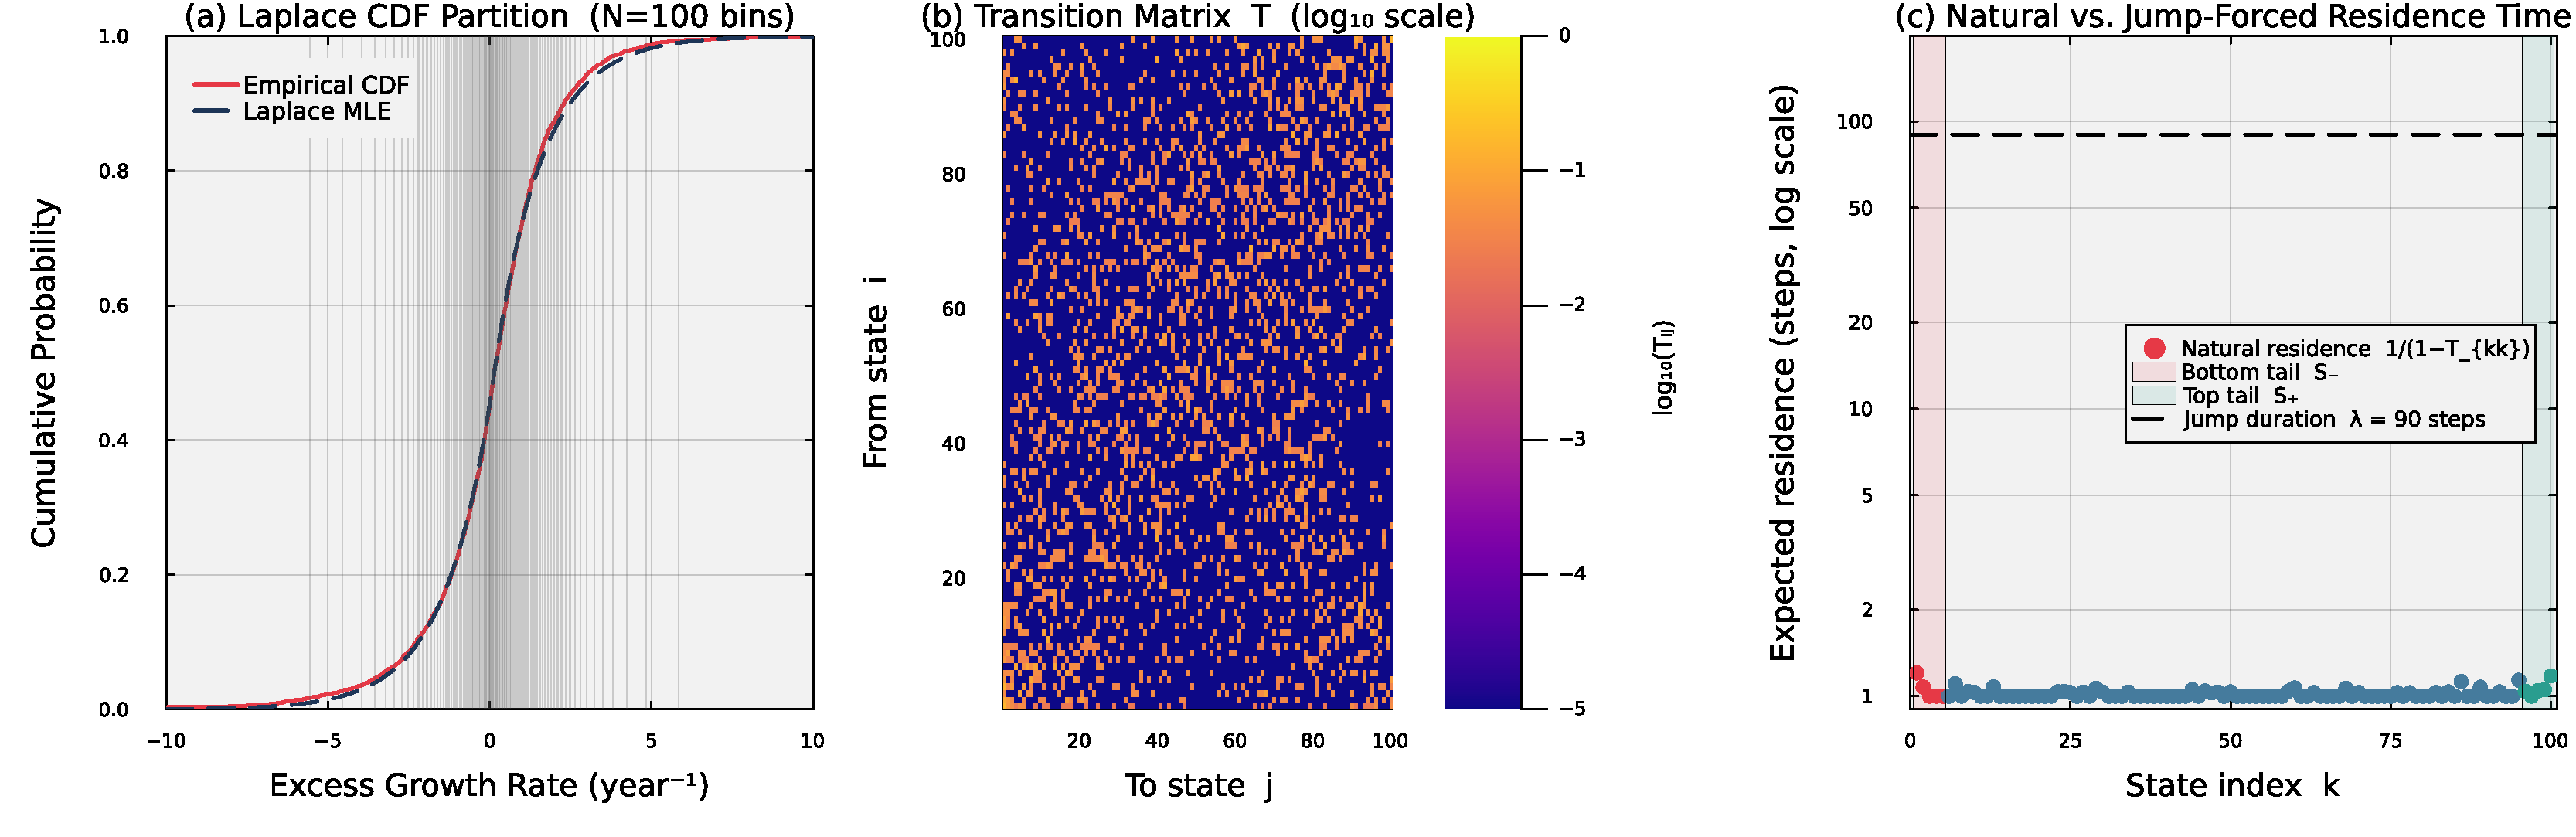
\includegraphics[width=\textwidth]{figs/supplement/FigS05-Model-Internals.pdf}
  \caption{\textbf{Fitted hidden Markov model with jumps (HMM-WJ)
    internals for SPY with $N = 100$ states.} Panel~(a) overlays the
    fitted Laplace cumulative distribution function (CDF) on the empirical
    CDF; the $99$ vertical lines mark the equal-probability quantile
    boundaries $Q_k$ that define the hidden states. Panel~(b) displays
    the estimated transition matrix $\mathbf{T}$ in $\log_{10}$ color
    scale; the dominant near-diagonal band reflects short-range regime
    persistence. Panel~(c) plots the expected natural residence time
    $1/(1 - T_{kk})$ for each state on a $\log_{10}$ scale, with the
    bottom tail set $\mathcal{S}_{-}$ (states $1$--$5$, red) and the
    top tail set $\mathcal{S}_{+}$ (states $96$--$100$, teal)
    highlighted. The dashed horizontal line marks the fitted
    mean jump duration $\lambda = 90$ steps, quantifying the
    two-order-of-magnitude gap between natural residence times and the
    jump-duration override.}
  \label{fig:model_internals}
\end{figure}

\section{Emission distribution and semi-Markov comparison}
\label{sec:supp-emission-hsmm}

To compare the emission and duration specifications, we evaluated
three variants on SPY
(Table~\ref{tab:emission_hsmm}): a hidden semi-Markov model (HSMM)
baseline adapted from Bulla and Bulla \cite{bullaBulla2006} ($K = 8$ states,
negative-binomial dwell times with a geometric fallback, and
Student-$t$ emissions), HMM-WJ with the original
Gaussian emissions ($N = 100$), and HMM-WJ with Student-$t$
emissions ($N = 100$). Both HMM-WJ variants had higher in-sample KS
and AD pass rates than the HSMM-style baseline. The HMM-WJ
variants use $100$ states and the HSMM uses $8$, so this comparison
does not assign the pass-rate difference solely to the duration
model. Holding the rest of HMM-WJ fixed, changing the emission from
Normal to Student-$t$ ($\nu=5$) increased simulated excess kurtosis
from $5.5$ to $7.5$, against an observed value of $7.7$. The Student-$t$
emission also increased the KS and AD pass rates, while ACF-MAE and
the distributional distances changed modestly. The emission choice
therefore explained the kurtosis gain in this controlled HMM-WJ
comparison, while it changed temporal fit little.

\begin{table}[H]
\centering
\caption{\textbf{Three-way comparison of emission distributions and
    duration specifications for SPY.} Standard
    errors in parentheses; bold marks the best value per row. The HSMM
    is a hidden semi-Markov-style model adapted from Bulla and Bulla
    ($K = 8$ states, negative-binomial dwell times with a geometric
    fallback, and Student-$t$ emissions) \cite{bullaBulla2006}; HMM-WJ:
    hidden Markov model with jumps
    ($N = 100$). All entries are computed from $1{,}000$ simulated
    paths at significance level $\alpha = 0.05$. Kolmogorov--Smirnov
    (KS), Anderson--Darling (AD), and mean absolute error in the
    autocorrelation function (ACF-MAE) are defined in
    Section~\ref{sec:supp-validation}.}
\label{tab:emission_hsmm}
\small
\begin{tabular}{@{}lccc@{}}
\toprule
\textbf{Metric} & \textbf{HSMM} & \textbf{HMM-WJ} & \textbf{HMM-WJ} \\
                & \textbf{(Student-$t$)} & \textbf{(Gaussian)} & \textbf{(Student-$t$)} \\ \midrule
States              & $K = 8$ & $N = 100$ & $N = 100$ \\[4pt]
\multicolumn{4}{l}{\textit{In-sample ($2{,}766$ trading days, $2014$--$2024$)}} \\[2pt]
KS pass rate (\%)   &  $82.0$ ($1.2$)         &  $97.0$ ($0.5$)         & $\mathbf{98.3}$ ($0.4$) \\
AD pass rate (\%)   &  $42.5$ ($1.6$)         &  $90.5$ ($0.9$)         & $\mathbf{94.8}$ ($0.7$) \\
Excess kurtosis     &   $4.8$ ($0.08$)        &   $5.5$ ($0.03$)        & $\mathbf{7.5}$ ($0.09$) \\
ACF-MAE             & $0.059$ ($<\!0.001$)    & $\mathbf{0.052}$ ($<\!0.001$) & $0.053$ ($<\!0.001$) \\
Wasserstein-$1$     & $0.176$ ($0.001$)       & $0.101$ ($0.002$)       & $\mathbf{0.097}$ ($0.001$) \\
Hellinger           & $0.113$ ($<\!0.001$)    & $0.076$ ($<\!0.001$)   & $\mathbf{0.074}$ ($<\!0.001$) \\[4pt]
\multicolumn{4}{l}{\textit{Out-of-sample ($249$ trading days, $2025$)}} \\[2pt]
KS pass rate (\%)   & $\mathbf{96.2}$ ($0.6$) &  $95.0$ ($0.7$)         &  $95.4$ ($0.7$) \\
AD pass rate (\%)   & $\mathbf{96.7}$ ($0.6$) &  $95.9$ ($0.6$)         &  $95.3$ ($0.7$) \\
Excess kurtosis     &   $4.1$ ($0.13$)        &   $4.9$ ($0.08$)        & $\mathbf{6.2}$ ($0.15$) \\
ACF-MAE             & $0.042$ ($<\!0.001$)    & $\mathbf{0.040}$ ($<\!0.001$) & $\mathbf{0.040}$ ($<\!0.001$) \\
Wasserstein-$1$     & $0.287$ ($0.002$)       & $\mathbf{0.275}$ ($0.005$) & $\mathbf{0.275}$ ($0.005$) \\
Hellinger           & $0.239$ ($0.001$)       & $0.212$ ($0.001$)       & $\mathbf{0.210}$ ($0.001$) \\
\bottomrule
\end{tabular}
\end{table}

% =============================================================================
% S7 State-resolution sensitivity
% =============================================================================

% --- Table: Hybrid composer broken out by branch ---
\begin{table}[H]
  \centering
  \caption{\textbf{Hybrid composition method broken out by branch.}
    $N_{\mathrm{tickers}}$: number of tickers assigned to each branch by
    the $R^2_{\mathrm{preserve}} = 0.80$ threshold. The clipped
    variance-preserving branch does not trigger anywhere in the
    universe ($\rho_i < 0.90$ for all tickers) and is omitted. The
    two trackers in the $R^2$-preserving branch (QQQ and SPYG) had
    median absolute errors of $0.005$ for $\beta$ and $0.001$ for
    $R^2$, with a KS pass rate of $100\%$.}
  \label{tab:branch}
  \small
  \begin{tabular}{lrrrrrr}
\toprule
Branch & $N_{\mathrm{tickers}}$ & $|\hat\beta-\beta|$ & $|\hat R^2 - R^2_{\real}|$ & KS pass (\%) & $W_1$ & $\kappa$ \\
\midrule
\texttt{hybrid} & 421 & 0.018 & 0.021 & 73.5 & 0.250 & 7.142 \\
\texttt{r2-preserve} & 2 & 0.005 & 0.001 & 100.0 & 0.099 & 11.525 \\
\bottomrule
\end{tabular}

\end{table}

% --- Table: synthetic tracker grid ---
\begin{table}[H]
\centering
\caption{\textbf{Synthetic-tracker grid for the $R^2$-preserving
    branch.} The observed universe places only two tickers on this
    branch, so we generated synthetic trackers at each
    $(\beta_{\mathrm{true}}, R^2_{\mathrm{true}})$ cell, composed them
    with Algorithm~\ref{alg:hybrid}, and recovered
    $(\hat\beta, \hat R^2)$ by ordinary least squares. Entries are
    medians over $100$ replications per cell with cross-replication
    standard deviations in parentheses; the Kolmogorov--Smirnov (KS)
    pass rate is the fraction of replications whose two-sample test
    against the target marginal exceeds $p = 0.05$. Every cell was
    assigned to the $R^2$-preserving branch.}
\label{tab:tracker_grid}
\small
\begin{tabular}{@{}ccccc@{}}
\toprule
$\boldsymbol{\beta_{\mathrm{true}}}$ &
$\boldsymbol{R^2_{\mathrm{true}}}$ &
$\boldsymbol{\hat\beta}$ & $\boldsymbol{\hat R^2}$ &
\textbf{KS pass (\%)} \\ \midrule
$0.8$ & $0.80$ & $0.8006$ ($0.0072$) & $0.7998$ ($0.0044$) & $100.0$ \\
$0.8$ & $0.85$ & $0.8006$ ($0.0059$) & $0.8497$ ($0.0041$) & $100.0$ \\
$0.8$ & $0.90$ & $0.8004$ ($0.0048$) & $0.8999$ ($0.0028$) & $100.0$ \\
$0.8$ & $0.95$ & $0.7995$ ($0.0033$) & $0.9500$ ($0.0013$) & $100.0$ \\
$0.8$ & $0.99$ & $0.7999$ ($0.0016$) & $0.9901$ ($0.0003$) & $100.0$ \\ \midrule
$1.0$ & $0.80$ & $1.0003$ ($0.0089$) & $0.8017$ ($0.0052$) & $100.0$ \\
$1.0$ & $0.85$ & $0.9994$ ($0.0084$) & $0.8497$ ($0.0039$) & $100.0$ \\
$1.0$ & $0.90$ & $0.9999$ ($0.0065$) & $0.8999$ ($0.0026$) & $100.0$ \\
$1.0$ & $0.95$ & $1.0005$ ($0.0036$) & $0.9502$ ($0.0013$) & $100.0$ \\
$1.0$ & $0.99$ & $1.0000$ ($0.0018$) & $0.9900$ ($0.0003$) & $100.0$ \\ \midrule
$1.2$ & $0.80$ & $1.2007$ ($0.0126$) & $0.8001$ ($0.0048$) & $100.0$ \\
$1.2$ & $0.85$ & $1.2011$ ($0.0105$) & $0.8503$ ($0.0043$) & $100.0$ \\
$1.2$ & $0.90$ & $1.1996$ ($0.0081$) & $0.8994$ ($0.0027$) & $100.0$ \\
$1.2$ & $0.95$ & $1.1995$ ($0.0052$) & $0.9498$ ($0.0014$) & $100.0$ \\
$1.2$ & $0.99$ & $1.1998$ ($0.0025$) & $0.9900$ ($0.0003$) & $100.0$ \\
\bottomrule
\end{tabular}
\end{table}

\section{State-resolution sensitivity}
\label{sec:supp-sensitivity}

To test whether the results depended on state resolution, we swept the
partition over $N \in \{30, 60, 90, 100, 150, 200, 350\}$ and
re-evaluated the in-sample Kolmogorov--Smirnov (KS) and
Anderson--Darling (AD) pass rates and the mean absolute error in the
absolute-return autocorrelation function (ACF-MAE) for the hidden
Markov model with no jumps (HMM-NJ) and the hidden Markov model with
jumps (HMM-WJ), holding the tail-set size $N_{\rm tail}$ fixed
(Table~\ref{tab:sensitivity_n}). HMM-NJ was insensitive to the
partition: its pass rates moved by less than one percentage point and
its ACF-MAE was unchanged at the reported precision, as expected for a
model with no duration override whose behavior could depend on the
width of a tail state. HMM-WJ traded the two metrics against each other. Because
$N_{\rm tail}$ is fixed, a finer partition makes the tail set a
narrower quantile band, so each forced step lands further out, and
ACF-MAE improved from $0.057$ at $N = 30$ to $0.045$ at $N = 200$. The
same narrowing left fewer observations behind each tail state's
emission parameters, and the AD pass rate, which weights tail
discrepancies heavily, moved the other way, from $97.1\%$ at $N = 30$
to $82.8\%$ at $N = 200$. The intermediate values were not monotone,
which is consistent with re-running the $(\epsilon, \lambda)$ grid
search on a finite path ensemble at each $N$. At $N = 350$ several
quantile bins were never visited in the historical record, leaving the
corresponding emission parameters undefined. We adopted $N = 100$ for
all subsequent experiments as a midpoint that held the KS pass rate
above $98\%$ and the AD pass rate within a few percentage points of its
best value while capturing part of the ACF-MAE improvement.

% --- Table: state-resolution sensitivity ---
\begin{table}[H]
\centering
\caption{\textbf{Sensitivity of in-sample fit to the number of
    states $N$.} All entries are computed from $1{,}000$ simulated
    in-sample-length paths for SPY at significance level
    $\alpha = 0.05$, with the tail-set size $N_{\rm tail}$ and the
    remaining hyperparameters of Table~\ref{tab:hyperparams} held
    fixed and the $(\epsilon, \lambda)$ grid search re-run at each
    $N$ for the hidden Markov model with jumps (HMM-WJ). Standard
    errors in parentheses: binomial for pass rates, bootstrap
    ($B = 500$) for the mean absolute error in the absolute-return
    autocorrelation function (ACF-MAE). HMM-NJ denotes the hidden
    Markov model with no jumps. Values at $N = 100$ reproduce the
    corresponding entries of Table~\ref{tab:model_comparison}.}
\label{tab:sensitivity_n}
\small
\begin{tabular}{@{}lcccc@{}}
\toprule
\textbf{Model} & $\boldsymbol{N}$ & \textbf{KS pass (\%)} &
  \textbf{AD pass (\%)} & \textbf{ACF-MAE} \\ \midrule
HMM-NJ & $30$  & $99.3$ ($0.3$) & $97.8$ ($0.5$) & $0.059$ ($<\!0.001$) \\
HMM-NJ & $60$  & $99.5$ ($0.2$) & $98.5$ ($0.4$) & $0.059$ ($<\!0.001$) \\
HMM-NJ & $90$  & $99.3$ ($0.3$) & $98.6$ ($0.4$) & $0.059$ ($<\!0.001$) \\
HMM-NJ & $100$ & $99.3$ ($0.3$) & $98.2$ ($0.4$) & $0.059$ ($<\!0.001$) \\
HMM-NJ & $150$ & $99.1$ ($0.3$) & $98.7$ ($0.4$) & $0.059$ ($<\!0.001$) \\
HMM-NJ & $200$ & $99.2$ ($0.3$) & $98.3$ ($0.4$) & $0.059$ ($<\!0.001$) \\ \midrule
HMM-WJ & $30$  & $98.4$ ($0.4$) & $97.1$ ($0.5$) & $0.057$ ($<\!0.001$) \\
HMM-WJ & $60$  & $96.7$ ($0.6$) & $91.4$ ($0.9$) & $0.053$ ($<\!0.001$) \\
HMM-WJ & $90$  & $98.3$ ($0.4$) & $95.2$ ($0.7$) & $0.055$ ($<\!0.001$) \\
HMM-WJ & $100$ & $98.3$ ($0.4$) & $94.8$ ($0.7$) & $0.053$ ($<\!0.001$) \\
HMM-WJ & $150$ & $97.7$ ($0.5$) & $91.7$ ($0.9$) & $0.052$ ($<\!0.001$) \\
HMM-WJ & $200$ & $96.0$ ($0.6$) & $82.8$ ($1.2$) & $0.045$ ($0.001$) \\
\bottomrule
\end{tabular}
\end{table}


% =============================================================================
% S8 Cross-asset generalization (NVDA, JNJ, JPM)
% =============================================================================

% --- Figure: Branch map in (beta, R^2) space ---
\begin{figure}[H]
  \centering
  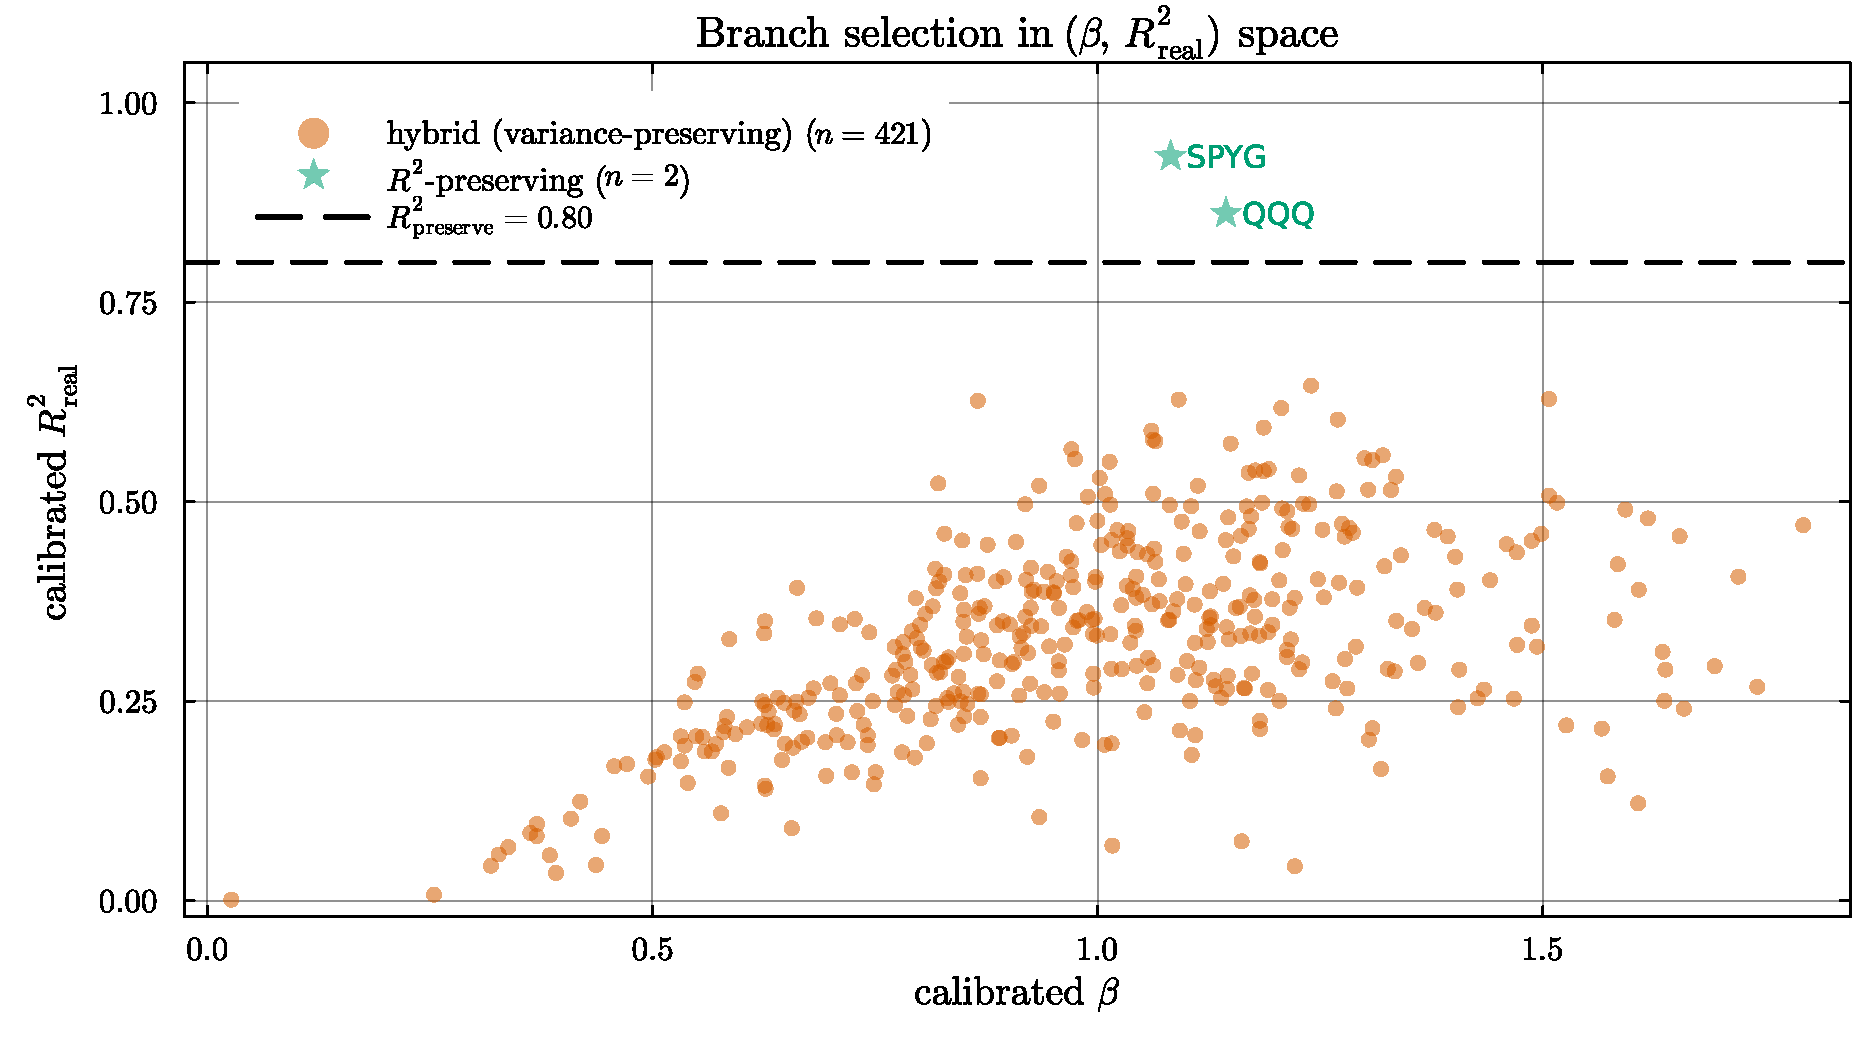
\includegraphics[width=0.85\textwidth]{figs/supplement/FigS06-Branch-Map.pdf}
  \caption{\textbf{Branch assignment in calibrated
    $(\beta, R^2_{\real})$ space.}
    The $R^2_{\mathrm{preserve}} = 0.80$ threshold (dashed line) separates
    tracker assets from single stocks. In this universe, only
    QQQ and SPYG exceed the threshold, and both are assigned to the
    $R^2$-preserving branch. The remaining $421$ tickers populate the
    variance-preserving branch; the clipped variance-preserving
    branch is unused because the market loading ratio
    $\rho_i = \beta_i^2 \sigma_m^2 / \sigma_{\gen,i}^2$ stays below
    $0.90$ for every ticker.}
  \label{fig:branch_map}
\end{figure}

% --- Table: Per-beta-bucket breakdown ---
\begin{table}[H]
  \centering
  \caption{\textbf{Aggregate metrics by $\beta$ quartile, across composition methods.}
    Quartile cutoffs are computed from the calibrated $\beta$ distribution
    across the $423$-ticker universe. The hybrid KS pass rate declines
    from $87.6\%$ in Q1 to $65.9\%$ in Q4 as the market loading ratio
    $\rho_i$ grows; the naive KS pass rate falls
    from $24.6\%$ to $1.3\%$ over the same range.}
  \label{tab:beta_bucket}
  \small
  \input{sections/tables/table3_by_beta_bucket}
\end{table}

% --- Table: Clipping-branch stress test ---
\begin{table}[H]
\centering
\caption{\textbf{Clipping-branch stress test under market-volatility
    scaling.} The market growth-rate path was rescaled by
    $\gamma \in \{1, 2, 3\}$ with the calibrated marginals held fixed,
    and the full hybrid composition method re-evaluated on the $423$-ticker
    universe. As $\gamma$ rises, the share of clipped tickers grows.}
\label{tab:stress}
\small
\begin{tabular}{@{}rr@{}}
\toprule
\textbf{$\gamma$} & \textbf{Clipped (\%)} \\ \midrule
$1$ & $0.0$  \\
$2$ & $76.4$ \\
$3$ & $95.2$ \\
\bottomrule
\end{tabular}
\end{table}

\section{Cross-asset generalization}
\label{sec:supp-cross-asset}

To test whether the single-asset procedure generalized beyond SPY, we
repeated the fitting and evaluation on three stocks: NVDA
(semiconductors, high volatility), JNJ (health care, low
volatility), and JPM (financials, moderate volatility). Per-ticker
tune outputs at $(n_{\mathrm{paths}} = 200, \mathrm{seed} = 1234)$
were reproducible with these settings (Table~\ref{tab:cross_asset}).
The objective combines
ACF and kurtosis errors with fixed weights. Because kurtosis varies
across finite samples of heavy-tailed paths, the selected grid point
can change with the Monte Carlo sample. The reported
$(\epsilon^{*},\lambda^{*})$ values are reproducible with the stated
path count and seed, but they are not unique per-ticker optima. At the
selected parameter values, in-sample HMM-WJ KS pass rates were
$98.9\%$ for NVDA, $99.4\%$ for JNJ, and $99.1\%$ for JPM.
Out-of-sample KS pass rates on the $249$-day $2025$ hold-out were
$97.7\%$, $74.0\%$, and $79.2\%$, respectively. Thus the strong
in-sample fit transferred unevenly across assets, especially on the
short holdout.

% --- Table: Cross-asset generalization ---
\begin{table}[H]
\centering
\caption{\textbf{Cross-asset generalization of the hidden Markov model
    with jumps (HMM-WJ) across three
    single-stock tickers spanning sector and volatility regimes.}
    Per-ticker tune outputs $(\epsilon^{*}, \lambda^{*})$ at
    $n_{\mathrm{paths}} = 200$ and $\mathrm{seed} = 1234$, and the
    corresponding HMM-WJ Kolmogorov--Smirnov (KS) and Anderson--Darling
    (AD) pass rates on $1{,}000$ simulated paths at $\alpha = 0.05$
    against each ticker's in-sample (IS; $2014$--$2024$) and out-of-sample
    (OoS; $2025$) growth-rate history. Values in parentheses are binomial
    standard errors (SEs) for pass rates. The
    $(\epsilon^{*}, \lambda^{*})$ values are reported as the parameter
    values used for the IS / OoS metrics rather than as canonical
    per-ticker optima.}
\label{tab:cross_asset}
\small
\begin{tabular}{@{}lcccccc@{}}
\toprule
\textbf{Ticker} & \textbf{$\epsilon^{*}$} & \textbf{$\lambda^{*}$}
  & \textbf{IS KS (\%)} & \textbf{IS AD (\%)}
  & \textbf{OoS KS (\%)} & \textbf{OoS AD (\%)} \\ \midrule
NVDA (semiconductors)    & $10^{-4}$ & $70$ & $98.9$ ($0.3$) & $96.7$ ($0.6$) & $97.7$ ($0.5$) & $96.1$ ($0.6$) \\
JNJ (health care)        & $10^{-4}$ & $70$ & $99.4$ ($0.2$) & $96.3$ ($0.6$) & $74.0$ ($1.4$) & $61.3$ ($1.5$) \\
JPM (financials)         & $10^{-4}$ & $80$ & $99.1$ ($0.3$) & $95.7$ ($0.6$) & $79.2$ ($1.3$) & $77.7$ ($1.3$) \\
\bottomrule
\end{tabular}
\end{table}

% --- Figure: R^2 distribution across the universe ---
\begin{figure}[H]
  \centering
  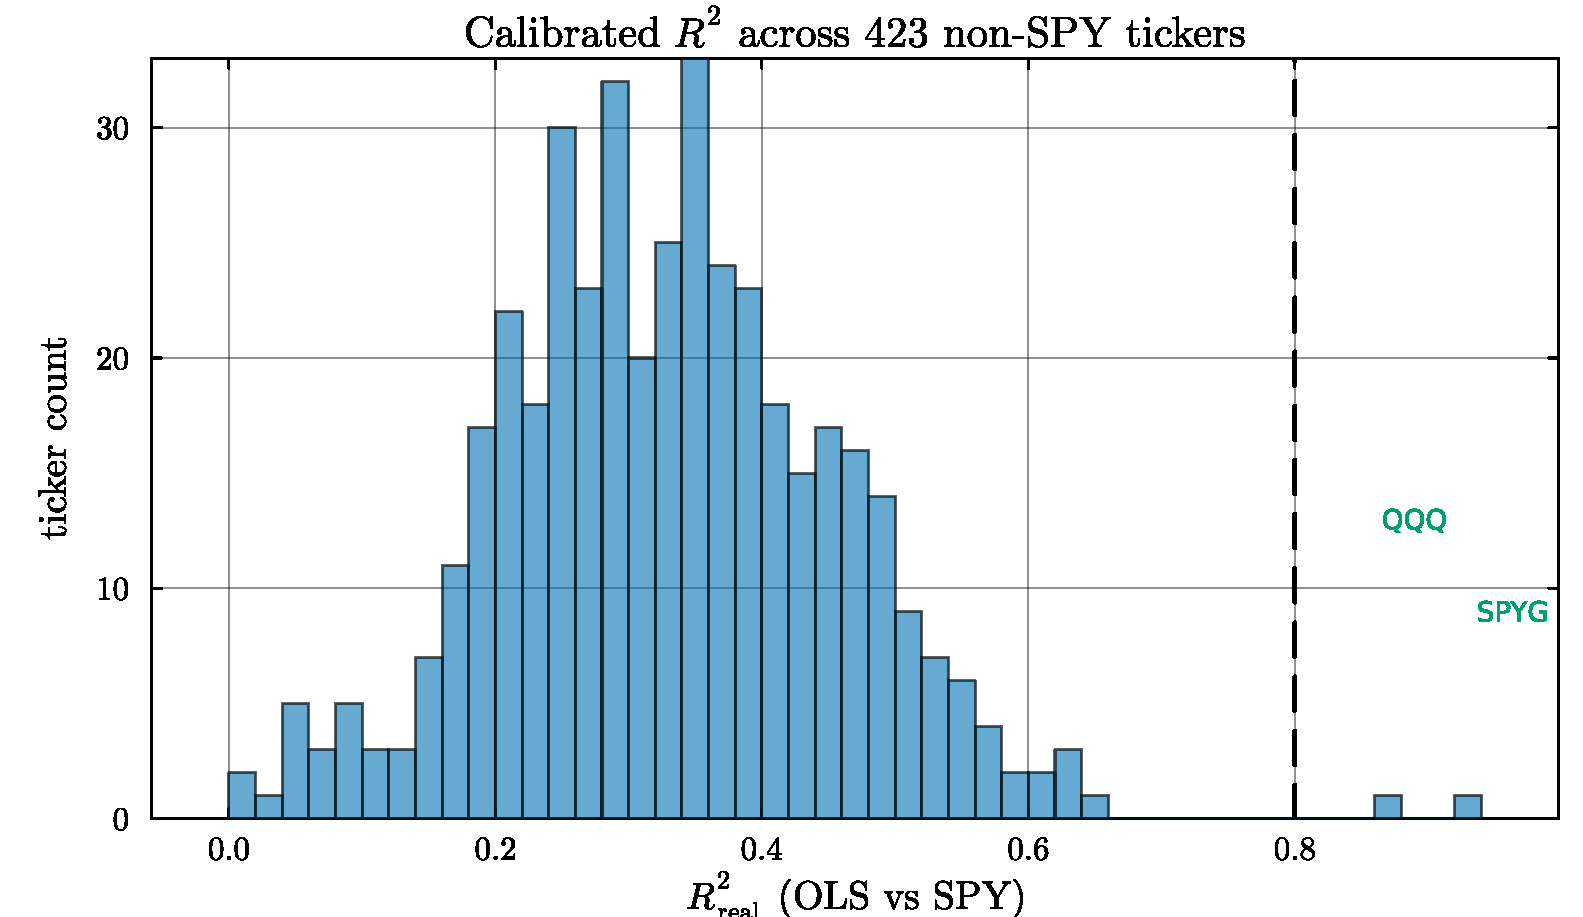
\includegraphics[width=0.85\textwidth]{figs/supplement/FigS03-R2-Distribution.pdf}
  \caption{\textbf{Calibrated $R^2$ distribution across the $423$
    non-SPY tickers.} Histogram of ordinary least-squares (OLS) $R^2$
    against SPY over the
    $2014$--$2024$ window. The two tickers crossing the
    $R^2_{\mathrm{preserve}} = 0.80$ threshold (dashed line) are index
    exchange-traded funds (QQQ, SPYG); the highest-$R^2$ individual
    stock (BLK, $0.645$)
    falls $\sim 0.16$ below the threshold. The $R^2$-preserving
    branch therefore contains only QQQ and SPYG in this universe.}
  \label{fig:r2_distribution}
\end{figure}

% --- Figure: Heavy-tail preservation ---
\begin{figure}[H]
  \centering
  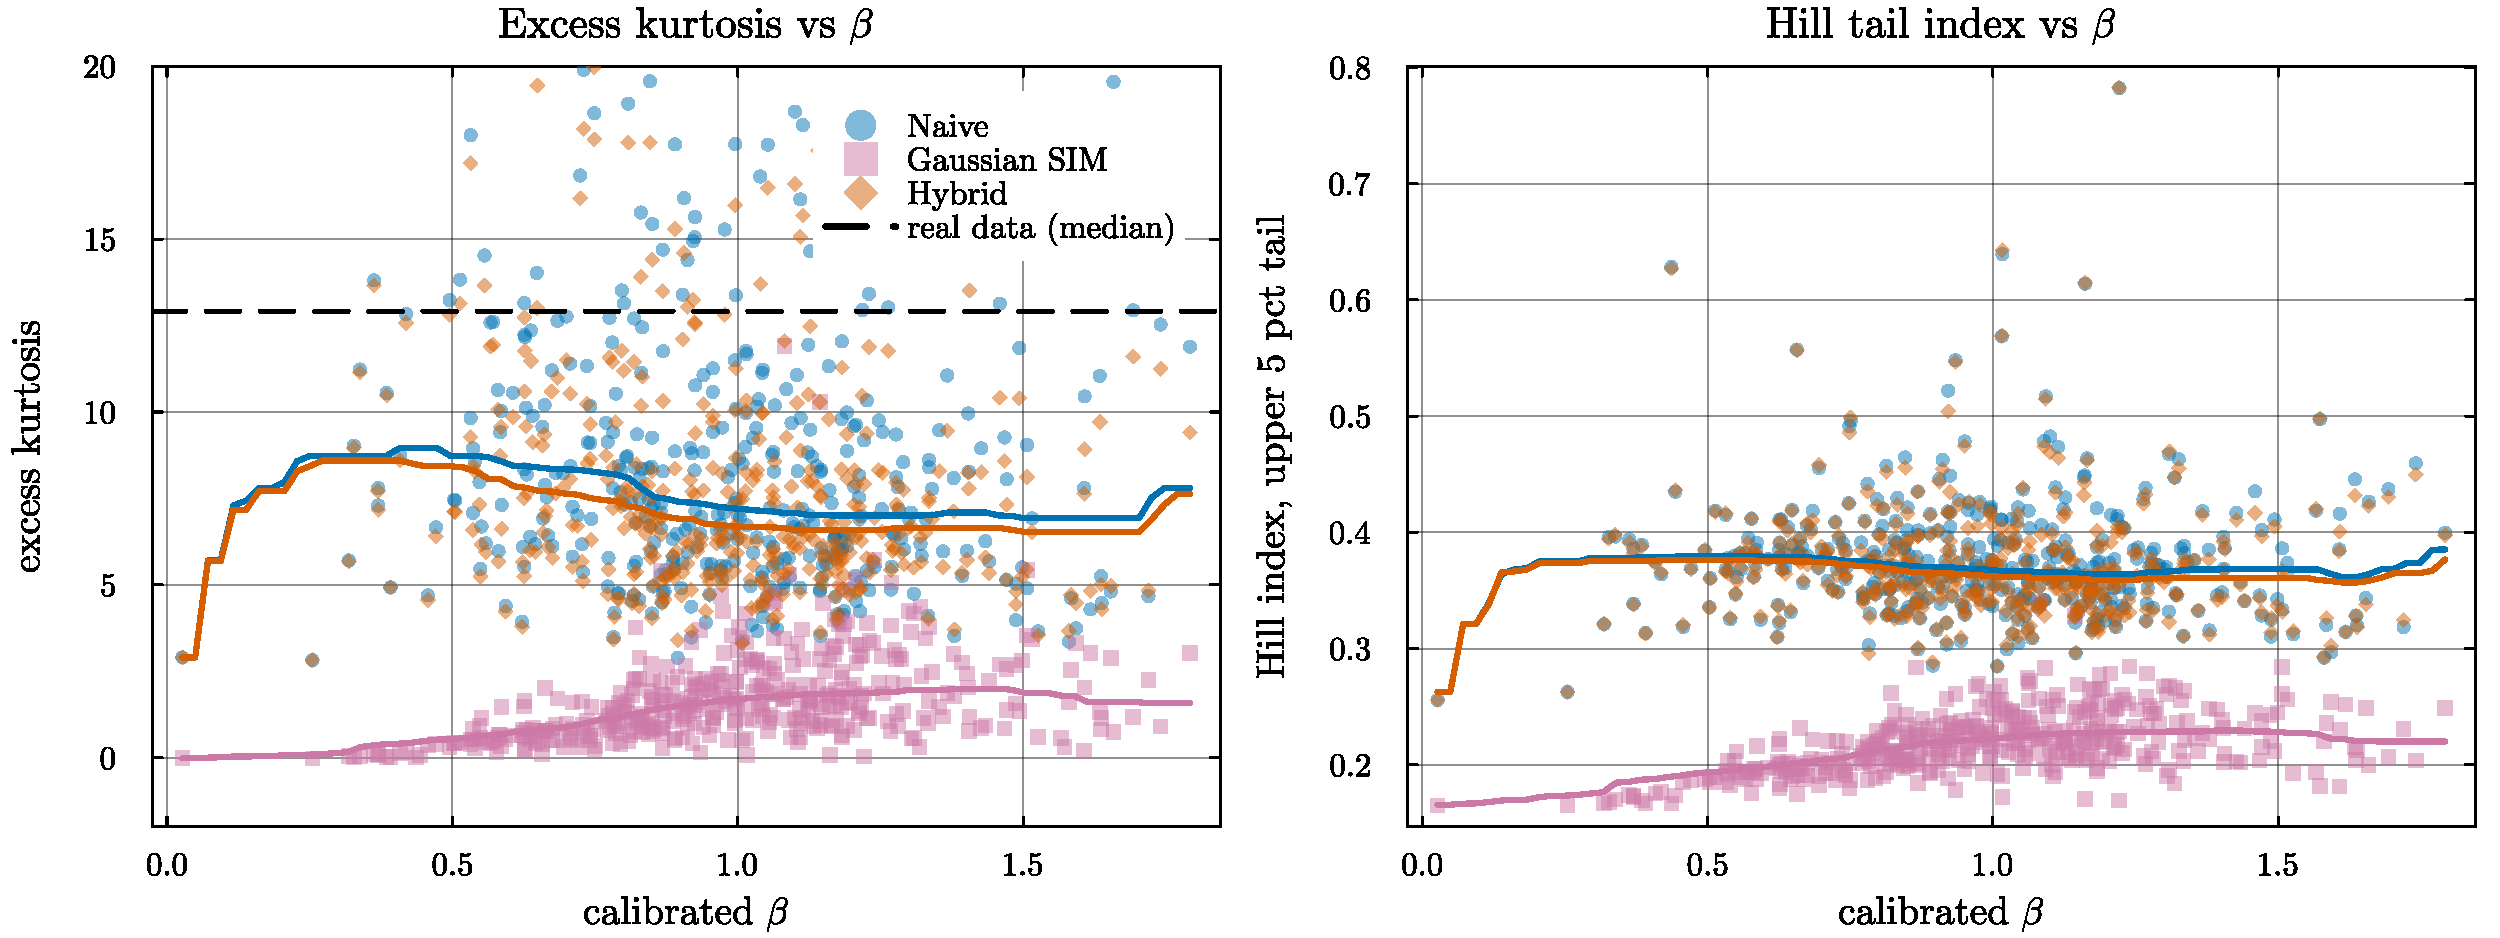
\includegraphics[width=\textwidth]{figs/supplement/FigS02-Tail-Preservation.pdf}
  \caption{\textbf{Heavy-tail preservation: excess kurtosis and Hill
    tail index vs calibrated $\beta$.}
    Each point is a per-ticker median over $100$ replications.
    \emph{Left:} excess kurtosis, $y$-axis clipped to $[-2, 20]$ for
    readability. The dashed line marks the median real-data excess
    kurtosis across the universe ($\kappa_{\real} \approx 13$); the
    hybrid and naive composition methods (orange and blue) track the generator's
    kurtosis, while the Gaussian single-index model (SIM) collapses to
    $\kappa \approx 1$.
    \emph{Right:} Hill tail-index estimator on the upper $5\%$ of
    $|g|$. The hybrid and naive medians remain near $0.37$ throughout the
    $\beta$ range; Gaussian SIM drops to $\sim 0.22$. The hybrid's median
    being below $\kappa_{\real}$ reflects the JumpHMM marginal's own
    kurtosis rather than a composition-rule distortion: hybrid tracks
    naive (both retain the generator's tails) while Gaussian SIM does not.}
  \label{fig:tails}
\end{figure}

\section{SIM composition derivations and properties verification}
\label{sec:supp-sim-derivations}

To verify the two closed-form targets used by the variance-corrected
single-index composition, we derived the variance scale of
Eq.~\eqref{eq:scale}, the residual-variance target of
Eq.~\eqref{eq:r2-target}, and the resulting large-$T$ OLS coefficients
and composed variance. To derive Eq.~\eqref{eq:scale}, first center the full-return
draw as in Eq.~\eqref{eq:center-generator}, then set
$\eps_i=s_i\tg_i^{\mathrm c}$ for $s_i\in[0,1]$ and require
that the composed series have the same variance as the generator
path:
\begin{equation}
  \Var(g_i) \;=\; \Var(\alpha_i + \beta_i\, g_m + \eps_i)
            \;=\; \Var(\beta_i\, g_m + \eps_i)
            \;=\; \sigma_{\gen,i}^2,
\end{equation}
where $\alpha_i$ drops out because it is constant. Expanding the sum
gives:
\begin{equation}
  \Var(\beta_i\, g_m + \eps_i) \;=\; \beta_i^2\, \Var(g_m)
  \;+\; 2 \beta_i\, \Cov(g_m,\, \eps_i)
  \;+\; \Var(\eps_i).
\end{equation}
Substituting $\eps_i = s_i\,\tg_i^{\mathrm c}$ gives
$\Var(\eps_i) = s_i^2\,\sigma_{\gen,i}^2$ and
$\Cov(g_m,\, \eps_i) = s_i\,\Cov(g_m,\, \tg_i^{\mathrm c})$. Under the
assumption $\Cov(\tg_i^{\mathrm c},\,g_m)\approx0$, the cross term vanishes and
the variance condition becomes
$\beta_i^2\, \sigma_m^2 + s_i^2\, \sigma_{\gen,i}^2 =
\sigma_{\gen,i}^2$. Solving for $s_i^2$ gives Eq.~\eqref{eq:scale}.

To derive Eq.~\eqref{eq:r2-target}, use the same zero-cross-covariance
assumption and write the population $R^2$ identity for
Eq.~\eqref{eq:sim-composition}:
\begin{equation}
  R^2 \;=\; \frac{\beta_i^2\, \sigma_m^2}{\beta_i^2\, \sigma_m^2 + \sigma_{\eps,i}^2}.
\end{equation}
Solving this identity for the residual variance gives
Eq.~\eqref{eq:r2-target}.
Because $\overline{\eps}_i=0$ after centering and scaling, the sample
mean of a composed path obeys
$\overline{g}_i=\alpha_i+\beta_i^{\eff}\overline{g}_m$. Hence, the
finite-sample OLS intercept was:
\begin{equation}
  \hat\alpha_i
  = \overline{g}_i-\hat\beta_i\overline{g}_m
  = \alpha_i-(\hat\beta_i-\beta_i^{\eff})\overline{g}_m.
\end{equation}
Under the zero-cross-covariance assumption, in the large-$T$ limit OLS
therefore gives $\hat\alpha_i \to \alpha_i$ and
$\hat\beta_i \to \beta_i^{\eff}$. Here
$\beta_i^{\eff}=\beta_i$ unless Eq.~\eqref{eq:clip} clips the market
loading. On the variance-preserving branch, the composed variance is
$\sigma_{\gen,i}^2$. Without clipping,
$\Var(g_i) = \beta_i^2 \sigma_m^2 + s_i^2 \sigma_{\gen,i}^2
  = \sigma_{\gen,i}^2$. Under clipping, Eq.~\eqref{eq:clip} sets
$\beta_i^{\eff}$ to give the same variance. On the $R^2$-preserving
branch, the composed variance is
$\beta_i^2 \sigma_m^2 / R^2_{i,\real}$, the value implied by the
calibrated $(\beta_i, R^2_{i,\real})$ rather than by the generator
marginal. On the ordinary-stock branch, the floor guarantees only that
$\Var(\eps_i)\geq f\,\sigma_{\gen,i}^2$; it does not guarantee that
adding the market term preserves the generator's tail distribution.
The KS pass rate fell from $87.6\%$ in the lowest-beta quartile to
$65.9\%$ in the highest-beta quartile (Table~\ref{tab:beta_bucket}).

\subsection{Role of the centered full-return draw as the residual}
\label{sec:supp-residual-choice}

The hybrid composition places $\eps_i = s_i \tg_i^{\mathrm c}$, a
centered and rescaled draw of asset $i$'s full return, in the residual
slot of Eq.~\eqref{eq:sim-composition}. On its face this is a category
mismatch: the residual of a single-index decomposition is the
idiosyncratic component of the return, orthogonal to the market, while
$\tg_i^{\mathrm c}$ is distributed like the centered total return,
market-driven component included. This appendix states what the
substitution preserves exactly, what it preserves approximately, and
how the approximation degrades as the market loading grows.

The residual slot must supply three things: a zero mean, so that the
intercept and market term alone set the conditional mean; the variance
$\sigma_{\gen,i}^2 - \beta_i^2 \sigma_m^2$ not already contributed by
the market term; and the asset-specific distributional shape, the
heavy tails and volatility clustering that motivated the single-asset
generator. Centering meets the first requirement exactly
(Eq.~\eqref{eq:center-generator}), the scale of Eq.~\eqref{eq:scale}
meets the second exactly, and the large-$T$ limits
$\hat\alpha_i \to \alpha_i$ and $\hat\beta_i \to \beta_i^{\eff}$ hold
because the draw is generated independently of the simulated market
path (Sec.~\ref{sec:supp-cov}), so the recovered factor structure is
exact as well. Any zero-mean, correctly scaled, market-independent
draw satisfies the first two requirements; the full-return draw is
chosen for the third, because it carries the per-asset marginal that
the single-asset validation certified. Only the shape requirement is
met approximately, and two exact statements bracket the
approximation.

At $\rho_i = 0$ the substitution is not an approximation:
Eq.~\eqref{eq:scale} gives $s_i = 1$, the market term contributes no
variance, and the composed series is the generator draw itself, so the
composed distribution equals the validated single-asset marginal. For
$\rho_i > 0$ the composed return is the sum of two independent
centered draws, and the survival of the generator's shape follows in
closed form. In population, conditional on the fitted parameters,
write the deviation of the composed return from its mean as
$X_m + X_i$, where $X_m = \beta_i\, g_m^{\mathrm c}$ is the market
contribution, $g_m^{\mathrm c}$ is the market path centered at its
mean, and $X_i = s_i\, \tg_i^{\mathrm c}$ is the scaled asset draw;
their variances are $v_m = \rho_i\, \sigma_{\gen,i}^2$ and
$v_i = (1 - \rho_i)\, \sigma_{\gen,i}^2$. Independence factors every
cross term in the fourth moment:
\begin{align}
  \E\big[(X_m + X_i)^4\big]
   &\;=\; \E(X_m^4) + 4\,\E(X_m^3)\,\E(X_i)
     \notag \\
   &\qquad + 6\,\E(X_m^2)\,\E(X_i^2)
     + 4\,\E(X_m)\,\E(X_i^3)
     \notag \\
   &\qquad + \E(X_i^4)
     && \text{(independence)} \notag \\
   &\;=\; \E(X_m^4) + 6\, v_m\, v_i + \E(X_i^4).
     && \text{($\E X_m = \E X_i = 0$)}
  \label{eq:supp-comp-fourth}
\end{align}
Writing $\kappa_m$ and $\kappa_{\gen}$ for the excess kurtosis of the
market path and of the generator draw, the component fourth moments
are $\E(X_m^4) = (\kappa_m + 3)\, v_m^2$ and
$\E(X_i^4) = (\kappa_{\gen} + 3)\, v_i^2$, where rescaling by $s_i$
leaves excess kurtosis unchanged. The excess kurtosis of the composed
return follows by dividing Eq.~\eqref{eq:supp-comp-fourth} by the
squared total variance:
\begin{align}
  \kappa(X_m + X_i)
   &\;=\; \frac{(\kappa_m + 3)\, v_m^2 + 6\, v_m\, v_i
     + (\kappa_{\gen} + 3)\, v_i^2}{(v_m + v_i)^2} \;-\; 3
     \notag \\
   &\;=\; \frac{\kappa_m\, v_m^2 + \kappa_{\gen}\, v_i^2
     + 3\, (v_m + v_i)^2}{(v_m + v_i)^2} \;-\; 3
     && \text{(collect terms)} \notag \\
   &\;=\; \kappa_m\, \rho_i^2 \;+\; \kappa_{\gen}\, (1 - \rho_i)^2.
     && \text{($v_m + v_i = \sigma_{\gen,i}^2$)}
  \label{eq:supp-kurt-comp}
\end{align}
The generator's excess kurtosis survives composition with weight
$(1 - \rho_i)^2$ and the market path's enters with weight $\rho_i^2$;
a simulation check with independent generator draws matched
Eq.~\eqref{eq:supp-kurt-comp} to within $0.03$ in mean excess
kurtosis at $\rho_i \in \{0.1, 0.3, 0.5\}$. For a low-loading asset
the composed tails are essentially the generator's: at
$\rho_i = 0.10$ the generator's kurtosis retains weight $0.81$. As
$\rho_i$ grows the composed shape moves away from the asset's own
marginal, which is the pattern in the documented diagnostics: the
hybrid tracks the generator's kurtosis across the $\beta$ range while
the Gaussian SIM does not (Fig.~\ref{fig:tails}), and the hybrid KS
pass rate declines from the lowest to the highest $\beta$ quartile
(Table~\ref{tab:beta_bucket}).

The residual-fit methods provide the exact-orthogonal alternative:
they fit a generator to each asset's OLS residual series, contain no
market component to double count, and are compared with the hybrid
in Table~\ref{tab:aggregate}; fitting JumpHMM to residuals requires
converting each residual series to a synthetic price path by
cumulative compounding and a second fit per asset. In summary,
$\tg_i^{\mathrm c}$ is not a residual in the orthogonal-decomposition
sense; it is a carrier of the validated marginal shape. The
substitution fixes the mean, the variance, and the recovered factor
loadings exactly, reproduces the asset's marginal exactly in the
$\rho_i \to 0$ limit, and dilutes the generator's shape with weight
$(1 - \rho_i)^2$ as the market share grows; the clipped and
$R^2$-preserving branches of Algorithm~\ref{alg:hybrid} handle the
region where the dilution is largest.
